% options:
% thesis=B bachelor's thesis
% thesis=M master's thesis
% czech thesis in Czech language
% slovak thesis in Slovak language
% english thesis in English language
% hidelinks remove colour boxes around hyperlinks

\documentclass[thesis=B,czech]{FITthesis}[2012/06/26]

\usepackage[utf8]{inputenc} % LaTeX source encoded as UTF-8


\usepackage{bbm}      %% \mathbbm
\usepackage{mathrsfs} %% \mathscr
\usepackage{amssymb}  %% matematicka symboly   
\usepackage{graphicx} %graphics files inclusion
\usepackage{alltt}
\usepackage{amsmath} %advanced maths
\usepackage{amssymb} %additional math symbols
\usepackage{multirow}
\usepackage{url}
\usepackage{dirtree} %directory tree visualisation

% % list of acronyms
% \usepackage[acronym,nonumberlist,toc,numberedsection=autolabel]{glossaries}
% \iflanguage{czech}{\renewcommand*{\acronymname}{Seznam pou{\v z}it{\' y}ch zkratek}}{}
% \makeglossaries

\DeclareMathOperator{\var}{var}						% Variance
\DeclareMathOperator{\cov}{cov}						% Covariance

\newcommand{\tg}{\mathop{\mathrm{tg}}} %cesky tangens
\newcommand{\cotg}{\mathop{\mathrm{cotg}}} %cesky cotangens

% % % % % % % % % % % % % % % % % % % % % % % % % % % % % % 
% ODTUD DAL VSE ZMENTE
% % % % % % % % % % % % % % % % % % % % % % % % % % % % % % 

\department{Katedra softwarového inženýrství}
\title{Webová demonstrace základních statistických výpočtů s~využitím matematického software R a SAGE}
\authorGN{Jana} %(křestní) jméno (jména) autora
\authorFN{Ernekerová} %příjmení autora
\authorWithDegrees{Jana Ernekerová} %jméno autora včetně současných akademických titulů
\supervisor{Ing. Daniel Vašata}

%ABSTRAKT BP
%slouží čtenáři k~rozhodnutí, zda vůbec bude text číst - první věc, kterou si čtenář přečte
%stručné shrnutí vaší BP
%rozsah cca 10 řádek
%nepoužívejte zkratky či odborné termíny bez vysvětlení - určeno pro~"průměrně vzdělaného čtenáře"
%nepoužívejte vycpávková slova a zbytečné výrazy
%nepoužívejte podmiňovací způsob ... "rád bych, aby analýza prokázala ..."
%nepoužívejte citové zabarvení - "je mi líto, že se v~práci nepodařilo", "mím radost, že analýza prokázala..."
%obvykle se píše v~minulém čase a trpném rodě

%CO, PROČ - JAKÝ PROBLÉM SE ŘEŠIL, JAKÝ JE CÍL TEXTU: tato práce se zabývá(řeší)...;Cílem práce je...;v práci jsem se zaměřil na...

%JAK JE PROBLÉM VYŘEŠEN ČI CÍL NAPLNĚN, POUŽITÉ POSTUPY, METODY, TECHNOLOGIE, ...: zvolený problém jsem vyřešil pomocí...;v řešení bylo použito metody, postupu a analýzy;práce představuje algoritmus takový, který;data jsem zpracovával pomocí těchto nástrojů a provedl vyhodnocení takové

%JAKÉ JSOU KONKRÉTNÍ VÝSLEDKY, JAK DOBŘE JE PROBLÉM VYŘEŠEN: podařilo se dosáhnout úspěšnosti 84% ; v~práci jsem vytvořil systém, který; vytvořené řešení poskytuje ty a ty možnosti; provedeným výzkumem bylo zjištěno, že

%ČÍM JE PRÁCE UŽITEČNÁ VĚDĚ ČI ČTENÁŘI(KOMUNITĚ): přínosem práce je; hlavním zjištěním je; hlavním výsledkem je; na~základě zjištěných údajů je možné; výsledký této práce umožňují

%ZÁVĚR: na~závěr práce je uvedeno; práce je doplněna o; v~příloze lze nalézt

\acknowledgements{V~první řadě bych chtěla poděkovat mému vedoucímu Ing.~Danielu Vašatovi za~skvělé vedení mé práce, cenné rady, nekonečnou trpělivost a ochotu odpovídat na~všechny moje otázky. Dále bych ráda poděkovala své rodině za~podporu během celého mého studia a svým přátelům, kteří jsou mi oporou a motivují mě v~mém studiu dál pokračovat.
}
\abstractCS{Tato práce se zabývá možnostmi integrace volně dostupných matematických algebraických systémů R a Sage do webové aplikace. Napojení statistického softwaru R do~webové aplikace bylo provedeno s~využitím API poskytovaného projektem OpenCPU, napojení matematického softwaru Sage za~pomoci služby Sage Cell Server. Oba zvolené matematické systémy se podařilo úspěšně využít ve~webové aplikaci postavené na~jazyce PHP. Výsledkem je jednoduchá webová aplikace pro~základní statistické výpočty. Hlavním přínosem práce je rozbor možností využití systémů R a Sage ve webové aplikaci a jejich porovnání z~hlediska jednoduchosti integrace, efektivity a praktické použitelnosti.}
\abstractEN{This thesis deals with options of the integration open source calculating algebraic systems R and Sage into~the~web application. The~connection of R software into~the~web application was done using API provided by OpenCPU project, the~connection of Sage was done with Sage Cell Server service. Both selected algebraic systems were successfully used in~the~web application built on PHP language. The~result is simple web application for basic statistical calculations. The~main contribution of this thesis is the analysis of the possibility of using software R and Sage in~the~web applications and their comparison in~terms of ease of integration, effectivity and practical applicability.  }
\placeForDeclarationOfAuthenticity{V~Praze}
\declarationOfAuthenticityOption{2} %volba Prohlášení (číslo 1-6)

%KLÍČOVÁ SLOVA
%odborné termíny, zkratky výstižně charakterizující obsah BP
%slouží k~vyhledávání - spolu s~abstraktem a názvem práce
%mohou být pojmy vyjádřené více slovy - sousloví či fráze (ne souvislé věty)
%pro potřeby BP postačuje 5-10 klíčových slov
%výčet klíčových slov se uvádí za sebou, oddělený čárkami
\keywordsCS{Webová aplikace, Základní statistické výpočty, Počítačový algebraický systém, Matematický software R, SageMath, PHP, OpenCPU, Sage Cell Server}
\keywordsEN{Web application, Basic statistical calculations, Computer Algebra System, Mathematical software R, SageMath, PHP, OpenCPU, Sage Cell Server}

\begin{document}

% \newacronym{CVUT}{{\v C}VUT}{{\v C}esk{\' e} vysok{\' e} u{\v c}en{\' i} technick{\' e} v~Praze}
% \newacronym{FIT}{FIT}{Fakulta informa{\v c}n{\' i}ch technologi{\' i}}

\begin{introduction}
	%sem napište úvod Vaší práce
	%VÝZNAM TÉMATU PRO SPOLEČNOST (KOMUNITU)
	%MOTIVACE VOLBY TÉMATU - PROČ SE TÉMATEM ZABÝVÁTE, PROČ JSTE SI JEJ ZVOLILI
	%ZAMĚŘENÍ PRÁCE - ZAŘAZENÍ TÉMATU BP DO SOUVISLOSTÍ - OKRUHY, KTERÝMI SE PRÁCE ZABÝVÁ (PŘÍPADNĚ NEZABÝVÁ); POSTUPY (METODY) POUŽITÉ V~PRÁCIŮ; PŘEDSTAVENÍ STRUKTURY PRÁCE (NÁVAZNOST JEDNOTLIVÝCH KAPITOL); NÁVAZNOST NA JINÉ BP
\subsection{Matematická statistika a web}
Matematická statistika jako vědní disciplína se od~počátku svého vývoje, na~začátku 18.století \cite{statistika}, rozšířila téměř do~všech empirických vědních disciplín. Počátky jejího vývoje jsou nejvíce spojovány s~přírodními vědami, jako je biologie, astronomie a psychologie, dnes má významnou roli také v~oblastech teorie měření, statistické fyziky, matematické lingvistiky, demografie a pojistné matematiky, ale také epidemiologie, robotiky a mnoha dalších. Tato oblast matematiky má široké využití nejen v~akademickém světě, ale také v~běžném životě. Hlavní úlohou statistiky je analýza dat obsahujících prvek nahodilosti. S~takovým vyhodnocením dat, tedy statistikou, se denně setkává každý, aniž si to mnohdy uvědomuje.  
%význam statistiky, že se dotýká nás všech, všech vědních disciplín, vídáme ji v~novinách, televizi, všude a pořád...

%co je to CAS a jaký má pro~nás význam
Počítačových algebraických systémů (anglicky Computer Algebra System - CAS) je již v~dnešní době velké množství. Jde zpravidla o~komplexní programy, které bývají účinným nástrojem k~počítání náročných úloh z~různých vědních disciplín. Některé z~těchto programů začínají pronikat také do~oblasti webových technologií a nabízejí různé způsoby online prezentace výpočtů i matematických demonstrací. Tyto systémy najdeme jak komerční, tak také Open Source. Tato bakalářská práce se zaměřovala výhradně na~Open Source systémy a to konkrétně software Sage a statistický software R.

%význam webu, že jsme všichni v~dnešní době neustále online a že je třeba statistiku moct počítat online...
Web má v~dnešní společnosti obrovský význam, nároky na~webové aplikace se čím dál více zvyšují a vyžadují složité analýzy online. Počítačové algebraické systémy byly k~takovým složitým analýzám vytvořeny, a tak je výhodné se pokusit je integrovat do webových aplikací a využít tak jejich vysoký analytický potenciál. 
%moje motivace k~výběru tématu

Autorčinou motivací k~výběru tohoto tématu pro~její bakalářskou práci byl hlavně velký zájem o~matematiku a touha spojit matematiku a informatiku do~jednoho uceleného projektu. Znalosti získané během tvorby této práce ji tak jistě budou nápomocné jak v~jejím dalším studiu, tak i v~budoucím zaměstnání.
	
\subsection{Cíle práce}


%cíl práce, čím se zabývá, všechny témata, které práce pokrývá, že je výsledkem i aplikace...

    Prvním cílem této bakalářské práce bylo prozkoumat možnosti integrace volně dostupných matematických systémů R a Sage do~webových aplikací.
    
    Z~tohoto důvodu se práce nejprve zabývá možnostmi napojení statistického software R do~webových prezentací s~využitím API poskytovaného projektem OpenCPU. V~další části pak obdobně možnostmi napojení matematického software Sage za~pomoci služby Sage Cell Server. Cílem analytické části práce také bylo prozkoumat závislost těchto řešení na~konkrétních webových technologiích.
    
    Dalším cílem a také cílem praktické části práce bylo navrhnout a vytvořit jednoduchou webovou aplikaci testující možnosti obou těchto systémů na~několika základních statistických úlohách.
    
    Posledním cílem práce poté bylo obě řešení otestovat a provézt jejich porovnání z~hlediska jednoduchosti integrace, efektivity a praktické použitelnosti.

\subsection{Struktura práce}
%struktura textu, čím se zabývají jednotlivé části práce
První část práce se věnuje analýze možností integrace R do~webových aplikací. Rozebírá možnosti, které pro~integraci můžeme využít a poté se zaměřuje na~analýzu API projektu OpenCPU. Analyzuje jeho přednosti a poté popisuje jak lze tento systém využívat.

V~druhé části obdobně analyzuje možnosti integrace Sage do~webových aplikací, zaměřuje se pak na~službu Sage Cell Server. Také rozebírá možnosti použití Sage ke statistickým výpočtům.

Další kapitola je poté věnována teorii k~vybraným metodám z~matematické statistiky, které jsou předmětem výpočtu v~testovací aplikaci.

V~poslední části se práce zabývá samotnou tvorbou aplikace, návrhu jednotlivých částí, integrací R a Sage do~webové aplikace a také implementací jednotlivých výpočtů. Na~závěr provedeme srovnání obou systémů.

\end{introduction}


%LITERÁRNÍ REŠERŠE - AKTUÁLNÍ STAV POZNÁNÍ V~DANÉ OBLASTI;
%ANALYTICKÁ ČÁST BP
%PŘEHLED O TOM, CO BYLO JIŽ V~DANÉ OBLASTI VYZKOUMÁNO
%HODNOCENÍ ZÁVĚRŮ, KTERÉ UČINILI JINÍ BADATELÉ
%NALEZENÍ MEZER, NEDOSTATKŮ, CHYB ...
%NÁPLŇ: DEFINICE POJMŮ, ANALÝZA TECHNOLOGIÍ, NÁSTROJŮ, METOD, POSTUPŮ, MATEMATICKÝCH PRINCIPŮ, STATISTICKÁ ANALÝZA, ...
%OBSAHUJE POUZE TÉMATA, KTERÁ BUDOU VYUŽITA PRO TVORBU VAŠÍ PRAKTICKÉ ČÁSTI PRÁCE
%
%OBOR WI:
%ANALÝZA UŽIVATELSKÝCH POŽADAVKŮ (POŽADAVKŮ ZADAVATELE); ANALÝZA PODNIKOVÝCH ČINNOSTÍ (PROCESŮ); ANALÝZA EXISTUJÍCÍCH APLIKACÍ, IS, PORTÁLŮ, ...; ANALÝZA POUŽITÝCH TECHNOLOGIÍ
\chapter[Analýza: R]{Analýza R a možnosti jeho použití ve~webové aplikaci - OpenCPU}
\section{Úvod do~R}
%co to je, kdy to vzniklo, proč, význam R, že je hojně využívaný,...
R je softwarové prostředí pro~statistické výpočty a grafiku. Při~dodržení podmínek GNU General Public License nadace Free Software Foundation je volně šířitelný a nevylučuje komerční využití programu. Jedná se o~projekt podobný jazyku a prostředí S vyvinutému v~Bell Laboratories (dříve AT\&T, nyní Lucent Technologies) Johnem Chambersem a jeho kolegy a lze ho považovat za~odlišnou implementaci jazyka S. Jsou mezi nimi některé významné rozdíly, ale většina kódu napsaného pro~S bude zároveň fungovat i~v~R \cite{rproject.org-about}.

Je multiplatformní - je dostupné pro~širokou škálu UNIXových prostředí, pro~Windows i MacOS X \cite{rproject.org}.  Zdrojové kódy a předkompilované verze programu R pro~nejběžnější operační systémy jsou dostupné na~stránkách nadace R Foundation for~Statistical Computing (CRAN).

R není jen prostředí, ale jde zároveň také o~jednoduchý a efektivní programovací jazyk obsahující podmínky, cykly, uživatelem definované rekurzivní funkce, prostředky pro~vstup a výstup. Kromě velkého množství statistických a grafických technik, poskytuje prostředky pro~manipulaci a ukládání dat, sadu operátorů pro~výpočty na~polích a maticích, rozsáhlé, konzistentní a integrované prostředky pro~analýzu dat, grafické prostředky pro~analýzu a zobrazování dat a to ať již na~obrazovce nebo v~tištěné podobě. Pomocí balíčků (\textit{packages}) je uživatelem velice snadno rozšiřitelné o~další metody. Přibližně osm balíčků je součástí oficiální distribuce R. Mnohé další balíčky pokrývající velmi rozsáhlou oblast moderní statistiky jsou dostupné přes~CRAN.

Snadnost, s~kterou lze vytvářet dobře navrhnuté obrázky a grafy patří k~největším přednostem tohoto prostředí. Do~grafů lze v~případě potřeby snadno vkládat matematické symboly a vzorce a uživateli je ponechána plná kontrola nad~výsledným vzhledem grafu. 

Další výhodou je možnost naprogramování výpočetně náročných postupů v~C, C++ nebo Fortranu a jejich následného připojení k~R a volání za~běhu~\cite{rproject.org-about}. 

R má také svůj vlastní, LaTeXu podobný, formát pro~tvorbu dokumentace, jenž je používán při~poskytování dokumentace on-line, či v~tištěné podobě a to hned v~několika formátech.

\section{Webové rozhraní pro~R}
%OpenCPU, Shiny a další možnosti...

Pro~R již bylo vyvinuto mnoho webových rozhraní. Několik možností lze nalézt na~stránkách samotného projektu R \cite{rproject.org-webInterfaces}. Informace na~těchto stránkách ale nejsou aktuální, a tak se situace již značně změnila. 

\begin{description}
\item[Rweb] \begin{sloppypar} Tento projekt byl vyvinut Jeffem Banfieldem, z~Montana State University, Montana, USA v~letech~1997-99 především pro~potřeby studentů statistiky na~této univerzitě \cite{Rweb}. \textit{Rweb} je sada webových stránek a Perl skriptů, které poskytují webové rozhraní založené na~R a které jeho autor nechává volně k~dispozici. Webové stránky tohoto projektu \cite{Rweb} a článek autora tohoto projektu vydaný v~roce 1999 v~internetovém periodiku Journal of Statistical Software \cite{RwebArticle} informují uživatele o~třech dostupných verzích tohoto rozhraní: základní Rweb, jenž od~svých uživatelů požaduje znalost jazyka R a který má běžet ve~většině prohlížečů, poté sofistikovanější verzi rozhraní v~jazyce Javascript a Rweb moduly. Všechny tři verze mají zároveň možnost načítání dat uživatele. Ty jsou webovým rozhraním načteny pomocí funkce R \textit{read.table}.\end{sloppypar}

Příklady užití v~článku autor dokládá obrázky a výstupy z~programu, poslední aktualizace stránek ale proběhla v~červnu 1999 a většina odkazů na~návody a dokumentaci nefunguje. Lze najít ještě stránky Jeana Thioulouse z~roku 2004 \cite{RwebJean}, které jsou celé postavené na~tomto webovém rozhraní, ale jejich zdrojové kódy jsou v~této době pravděpodobně jedinou dostupnou \uv{dokumentací} k~tomuto projektu, což ho v~zásadě činí nepoužitelným.

\item[R-Online] \begin{sloppypar} Webové rozhraní, které vytvořil Ulf Bartel. Jde ale o~podobný příklad jako předchozí projekt. Poslední aktualizace na~stránce proběhla v~roce 2005 a ačkoliv je v~dokumentaci (pouze v~němčině) napsáno o~mnoha funkcích, jediný odkaz na~příklad hlásí chybu na~serveru \cite{Ronline}.\end{sloppypar}

\item[Web Decomp, E-Decomp] \begin{sloppypar} \textit{Web Decomp} je statistický plugin pro~MS Excel a \textit{E-Decomp} webové rozhraní pro~R. Stránky projektu však nenabízí žádný funkční příklad použití a dokumentace k~webovému rozhraní je pouze v~japonštině \cite{WebDecomp}, což značně zužuje okruh potenciálních uživatelů.\end{sloppypar}

\item[Rserve, FastRWeb] \begin{sloppypar}Jde o~projekt Simona Urbanka. Jedná se o~TCP/IP server, který umožňuje využít prostředí R z~různých programovacích jazyků bez nutnosti jeho inicializace nebo odkazů na~R knihovnu. Každé připojení má zvlášť oddělený pracovní prostor a adresář. Implementace strany klienta je k~dispozici pro~rozšířené jazyky jako je C/C++, PHP nebo Java. \textit{Rserve} podporuje vzdálené připojení k~serveru, autentizaci a přenos souborů. Typické použití je integrování backendu R pro~výpočet statistických modelů, grafů a dalších funkcí v~různých aplikacích \cite{Rserve}.\end{sloppypar}

Verze \textit{Rserve} pro~použití na~webu se jmenuje \textit{FastRWeb}, má svoje vlastní webové stránky a dokumentaci, i když ne tak bohaté jako samotný Rserve. FastRWeb je infrastruktura, která umožňuje jakémukoliv webserveru použít R scripty pro~generování obsahu za~běhu, jako jsou webové stránky a grafika. URL jsou mapovány do~skriptů a mohou mít volitelné argumenty, které jsou poslány funkcím R běžícím ve skriptu. Například volání 
\begin{verbatim}
 http://my.server/cgi-bin/R/foo.png?n=100
 \end{verbatim} 
 by způsobilo, že FastRWeb zavolá funkci ve skriptu foo.png.R s~parametrem~n:  \begin{verbatim} fce_v_foo.png.R(n="100").\end{verbatim}
 FastRWeb může běžet na~jakémkoliv webserveru, který podporuje CGI (Common Gateway Interface) nebo PHP \cite{FastRWeb}. 
 
 Stránky Rserve byly naposledy aktualizovány v~roce 2013 a stránky FastRWeb v~roce 2012. Je možné zde najít několik odkazů na~aplikace využívající Rserve a psaných v~jazycích C/C++ nebo Javě, a také webové aplikace. Dokumentace, i když stručná nám poskytuje kompletní návod, jak tento projekt využít. 
 
\item[CGIwithR] \begin{sloppypar}Jedno z~webových rozhraní pro~R, o~kterých bylo publikováno v~elektronickém časopise Journal of Statistical Software. David Firth, autor projektu, v~článku \textit{CGIwithR: Facilities for processing web forms using R} \cite{CGIwithRArticle} seznamuje s~tímto balíčkem pro~použití se statistickým výpočetním prostředím R. Balíček má usnadňovat zpracovávání informací z~webových formulářů a zobrazování výsledků v~HTML přes CGI protokol. To je protokol určený pro~komunikaci mezi webovým serverem a programem generujícím dynamický obsah. CGIwithR umožňuje jednoduché použití R jako skriptovacího jazyka CGI, čímž uživateli zpřístupňuje rozsáhlé statistické zázemí prostředí R v~CGI skriptech, aniž by se musel nejprve učit jiné programovací jazyky, například Perl, který je pro~CGI skripty velice populární.\end{sloppypar} 

Stránky projektu neodkazují na~žádné online příklady, ale je zde několik ukázkových souborů, které jsou volně ke stažení \cite{CGIwithR}. A ačkoliv článek o~projektu v~Journal of Statistical Software je již z~roku 2003, poslední aktualizace na~webu projektu proběhla v~loňském roce (2014) a zdrojové kódy jsou k~dispozici ke stažení přímo na~jeho stránkách nebo na~GitHub.com. 

\item[Webbioc] \begin{sloppypar}\textit{Webbioc} byl součástí projektu \textit{Bioconductor} a poskytoval webové rozhraní pro~použití balíčků R vytvořených v~rámci tohoto projektu. Bioconductor je open source softwarový projekt poskytující nástroje pro~analýzu a porozumění genomickým datům (data spojená s~analýzou dědičné informace organismu - genomu \cite{slovnik}) a je založen především na~programovacím jazyce R. Na~webu projektu Bioconductor už ale nelze najít žádné informace o~tomto webovém rozhraní. Ačkoliv projekt Bioconductor je stále aktivní, poskytuje pouze R balíčky pro~výpočty spojené s~oblastí genetiky. \end{sloppypar}

\item[Rook, RApache, brew] \begin{sloppypar}Nástroje pro~R vytvořené Jeffreym Hornerem. Prvním z~nich je R balíček \textit{Rook}. Rook je webové rozhraní a zároveň softwarový balíček pro~R, který definuje rozhraní mezi webovým serverem a R aplikací. Aplikace Rook je doslova funkce R, která přijímá jako vstup prostředí R a vrací list příslušných HTTP položek (status, HTTP hlavičku a tělo HTML dokumentu) jako výstup \cite{Rook}.  Dalším autorovým počinem je \textit{RApache}, projekt podporující vývoj webových aplikací za použití prostředí a jazyka R a webového serveru Apache \cite{RApache}. A třetím, také nezanedbatelným projektem je balíček \textit{brew} pro~tvorbu zpráv, v~nichž může uživatel kombinovat souhrnné tabulky a grafy z~R s~rozsáhlými texty \cite{brew}.\end{sloppypar}

\item[Rwui] \begin{sloppypar}On-line aplikace, která se používá k~vytvoření webového rozhraní pro~běh R skriptu. Kód je generovaný automaticky, takže rozhraní pro~R skript může být stáhnuto a rozběhnuto během několika minut a uživatel nemusí mít žádné znalosti z~oblasti programování webových aplikací \cite{Rwui}. Autor skriptu vytvoří webovou aplikaci vyplněním informací v~sekvenci několika po sobě jdoucích webových formulářů, poté je mu vygenerovám kód aplikace, kterou si stáhne a nainstaluje na~vlastní server.\end{sloppypar}

\item[R-php] \begin{sloppypar}Projekt rozvíjený na~University of Palermo v~Itálii. Jeho autory jsou Angelo M. Mineo a Alfredo Pontillo a jeho cílem je vytvořit webově orientovaný statistický software. \textit{R-php} je vytvářen v~PHP a MySQL, je to volně šířitelný software s~všeobecnou veřejnou licencí GNU. Implementuje dva moduly: První umožňuje jednoduché vkládání kódu R a zobrazování výsledků (analýz a grafů) na~jiné stránce. Druhý modul provádí statistické analýzy za použití grafického uživatelského rozhraní. Projekt vznikl v~roce 2005 a není jasné, zda na~něm autoři stále pracují. Na~webu projektu najdeme jak příklady využití, tak kompletní dokumentaci v~italštině, a také v~angličtině \cite{R-php}. Využití R-php je však vhodné pouze v~aplikacích založených na~jazyce PHP.  \end{sloppypar}

\item[R PHP ONLINE] \begin{sloppypar}CGI webové rozhraní pro~chod R programů online, včetně grafického výstupu. Autorem je Steve Chen z~TKU, Taipei, Taiwan. Projekt je vydán pod veřejnou licencí a může být použit jak ve Windows, tak v~linuxovém prostředí. Jde o~čisté CGI rozhraní, kód R tedy není volán přes PHP knihovnu. Funguje tak, že nejprve deleguje program v~R do příslušného R balíčku a poté zobrazuje výstupy online  \cite{R_PHP_ONLINE}. Poslední novinka k~projektu je na~stránkách datována rokem 2003 a velká část webu je v~čínském jazyce.\end{sloppypar}

\item[Shiny] \begin{sloppypar}Framework pro~tvorbu webových aplikací v~R. Balíček shiny byl na~CRAN přidán teprve 20.února letošního roku~(2015), jde tedy o~poměrně nový projekt. Umožňuje velice snadné vytváření interaktivních webových aplikací s~R. Jeho součástí je mnoho ovládacích prvků pro~manipulaci s~daty (zaškrtávací a přepínací políčka, posunovače, tlačítka, výběrová pole, formuláře pro~textové i numerické vstupy a formuláře pro~vložení souborů) \cite{Shiny}. Interaktivita, kterou tento framework nabízí jinak statickému prostředí R a zároveň fakt, že uživatel nepotřebuje znát HTML, CSS, ani JavaScript patří k~jeho velkým přednostem. Naopak se ale uživatel musí seznámit se strukturou a jazykem shiny a samozřejmě znát jazyk R. Uživatel má možnost využít pro~své shiny aplikace online cloud. Tato služba je k~dispozici buď s~omezenými možnostmi zdarma, nebo v~různých úrovních placená. Na~placeném účtu má pak uživatel prostor pro~více aplikací, e-mailovou podporu, možnost autentifikace uživatelů při vstupu do jeho aplikací a hlavně možnost více hodin jejich aktivního užívání. Stejně tak si může uživatel vybrat ze dvou verzí serveru. Zdarma má k~dispozici ke stažení tzv. Open Source Edition verzi balíčku pro~instalaci serveru, placená je potom verze Professional Edition. Ta má samozřejmě zase více možností a vychytávek. Projekt není vhodný pro~použití z~externích webových aplikací.\end{sloppypar}

%\item[OpenCPU] API poskytované projektem OpenCPU.

\end{description}

\section{OpenCPU}

\subsection{Proč OpenCPU}
Je zřejmé, že používání R ve webových aplikacích se v~dnešní době těší vysoké oblibě, a uživatelům se tak již nabízí široké možnosti. Pro integraci statistického softwaru R do webové aplikace je v~této bakalářské práci použit \textit{OpenCPU} systém a to hned z~několika důvodů. 

Tento projekt nabízí HTTP API pro~použítí jazyka R ve webové aplikaci. Jde o~čisté spojení R a webu. OpenCPU je kompatibilní s~jakýmkoliv jazykem nebo frameworkem, který umožňuje komunikaci pomocí protokolu HTTP. Zároveň se uživatel nemusí učit žádný složitý nový jazyk, či systém, pouze propojuje funkce R se svou webovou aplikací. 

Narozdíl od většiny projektů z~předchozí kapitoly je OpenCPU projekt nový a stále se rozšiřuje. Web projektu nám nabízí kompletní, ucelenou a přehlednou dokumentaci a online běžící vzorové aplikace včetně možnosti stažení jejich zdrojových kódů. V~OpenCPU aplikaci můžeme použít jakékoliv funkce a balíčky R, můžeme použít funkce ostatních uživatelů OpenCPU, nebo si napsat vlastní. OpenCPU aplikace je vlastně balíček R, je tedy možné ho použít lokálně v~R, můžeme ho rozběhnout na~vlastním serveru, nebo použít jeden z~veřejných serverů, které OpenCPU poskytuje. 

Další nezanedbatelnou výhodou tohoto systému je, že je pro~všechny uživatele zcela zdarma a je také využitelný pro~komerční účely. 

\subsection{Seznámení s~OpenCPU}
Projekt vznikl jako součást (post) doktoranského výzkumu Jeroena Oomse na~katedře statistiky na~University of California v~Los Angeles, USA \cite{OpenCPU-Papers}. Verze 1.0 byla představena v~srpnu 2013 a od té doby bylo vydáno několik aktualizací. V~současné době (duben 2014) poslední aktualizace na~blogu autora pojektu uvádí verzi OpenCPU 1.4.6. \cite{OpenCPUreaease146}.

OpenCPU slouží pro~podporu on-line zabudovaných vědeckých výpočtů a reprodukovaných vědeckých výzkumů. OpenCPU server poskytuje spolehlivé a spolupráce schopné HTTP API pro~analýzu dat postavenou na~jazyce a prostředí R. Uživatelé mohou využít vlastní server, nebo server tímto projektem veřejně poskytovaný. Ten díky použití webhook obsahuje vždy nejaktuálnější verzi našeho balíčku. OpenCPU poskytuje také klientskou knihovnu JavaScriptu postavenou na~jQuery, která umožňuje volat funkce R za použití AJAXu.

Velmi diskutovaný je rozdíl mezi projektem Shiny a OpenCPU systémem. Hlavním rozdílem je účel, ke kterému tyto projekty slouží. Shiny je framework pro~tvorbu interaktivních webových demonstrací v~R, naproti tomu OpenCPU je API, tedy tvoří pouze most, který spojuje webovou část s~částí analytickou obsahující volané funkce R. 

OpenCPU je kompatibilní s~jakýmkoliv jazykem nebo frameworkem, který umožňuje komunikaci pomocí protokolu HTTP. Uživatel není omezen sadou dostupných panelů nebo widgetů. OpenCPU spravuje příchozí požadavky, bezpečnost, přidělování zdrojů, vstup a výstup dat a další technické náležitosti. Nic víc, nic míň. 

Rozdíl se systémem Shiny je také v~tom, jak klient udržuje spojení se serverem. V~Shiny podobně jako v~terminálu R jde o~klasický stavový protokol, tedy klient se serverem udržují neustálé spojení, relaci, a tak server pozná, že po sobě jdoucí požadavky spolu souvisí, tedy že pocházejí od stejného klienta. OpenCPU je ale čisté HTTP, tedy protokol bezestavový, a tak ačkoliv poskytuje funkce pro~relační objekty, funguje trochu jinak, než jsme u~stavových aplikací zvyklí. Po každém volání funkce, OpenCPU ukončí (případně zabije) R proces, který byl použit ke zpracování požadavku. Nicméně, všechny výstupy každého volání funkce, jako návratové hodnoty, grafika nebo soubory v~pracovním adresáři, jsou uloženy na~serveru a ID relace je vrácena klientovi. To může být poté použito v~budoucích HTTP požadavcích. Například může klient získat výstupy v~různých formátech, sdílet je s~ostatními, nebo použít uložené R objekty jako argumenty v~následujících voláních funkcí. Objekty nejsou nijak přiřazeny globálnímu prostředí a to má hned několik výhod: všechno je asynchronní, a tak GUI nebude blokováno během čekání na~výstup z~R; další výhodou je, že pokud se volání R zasekne, chybuje nebo havaruje, aplikace nespadne; aplikace díky tomuto provedení počítají už z~principu paralelně, klienti tedy mohou provádět požadavky současně a spojit jejich výstupy později \cite{OpenCPUjsLibrary}. 

Způsob, jakým jsou odděleny GUI a funkce R poskytují základy pro~týmovou spolupráci na~projektu. Je tak umožněno, že weboví vývojáři mohou použít jejich oblíbený jazyk pro~volání R funkcí přes HTTP. OpenCPU poskytuje most mezi těmito dvěma systémy, a tak se analytik, který vytváří funkce pro~datovou analýzu v~R nemusí vůbec zabývat vývojem webu a zároveň se webový vývojář vůbec nemusí dostat do styku s~jazykem R. Tyto dvě vrstvy jsou v~aplikaci naprosto odděleny.

Všechny části OpenCPU jsou zveřejněny pod licencí Apache2, může tak být šířen a upravován jako open source, nebo použit pro~komerční účely.

\section{Jak používat OpenCPU}
Tato sekce hovoří o~tom, jak OpenCPU používat, co všechno je k~jeho chodu potřeba, kam umístit funkce, které chce uživatel volat z~webové stránky a jak k~nim přistupovat. Sekce je rozdělena do několika podkapitol. První podkapitola je o~funkcích R, poté následuje serverová část a až nakonec část o~tom, jak k~funkcím přistupovat z~webové aplikace.   

\subsection{Funkce R}
Má-li uživatel již vlastní běžící webovou aplikaci, do nichž bude výpočty R integrovat, nebo s~tvorbou celé aplikace teprve začíná, každopádně bude muset zjistit, jaké funkce R k~jeho záměrům bude potřebovat. Není vždy nutné tvořit hned vlastní, je možné použít jakékoliv funkce z~veřejně dostupných balíčků. Pokud chce tvořit OpenCPU aplikaci, tedy balíček, který zároveň obsahuje webové stránky aplikace, vyžaduje OpenCPU k~udržení přehlednosti, aby byly v~této aplikaci použity pouze funkce z~tohoto balíčku. Pro použití funkcí z~jiných balíčků je nutné použít obalovací funkce a správně deklarovat závislosti na~těchto balíčcích. Princip obalovací funkce spočívá v~tom, že vlastně sama žádný výpočet nedělá, pouze volá funkci, případně funkce, které výpočet provádějí. Deklarovat závislosti je nutné v~souboru NAMESPACE, jenž je povinnou součástí každého R balíčku a dostaneme se k~němu později. Seznam dostupných balíčků na~veřejném serveru OpenCPU je k~dispozici zde: \url{https://demo.ocpu.io/}. 

Informace o~daném balíčku umístěném na~tomto serveru je možné najít na~adrese:
\begin{alltt}
https://demo.ocpu.io/\{název_balíčku\}/info
\end{alltt}
Tedy například na~adrese \url{https://demo.ocpu.io/A3/info} jsou informace o~balíčku \textit{A3}. Struktura tohoto výpisu je vidět na~obrázku 1.1 .

\begin{figure}[ht]
    \centering
    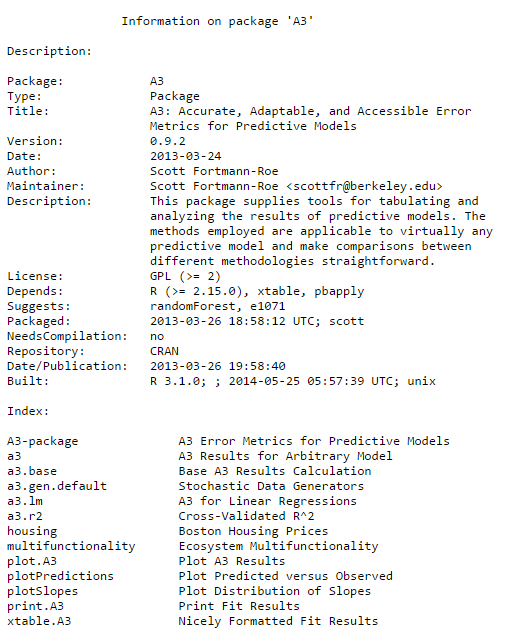
\includegraphics[scale=0.6]{grafics/packageInfo.PNG}
    \caption{Ukázka popisu balíčku R \cite{info}}
\end{figure}

Tato stránka s~popisem obsahuje informace obsažené v~souboru \textit{DESCRIPTION}, který je jednou z~povinných součástí každého R balíčku. Najdeme zde název, verzi, jméno autora, licenci, pod kterou je balíček zveřejněn, slovní popis funkcionalit, datum vydání a další nepovinné atributy. Pod základními charakteristikami balíčku je zobrazen výpis funkcí, které balíček obsahuje a u~každé popis této funkce z~její manuálové stránky. Seznam funkcí obsažených v~balíčku lze najít také na~stránce: 
\begin{verbatim}
https://demo.ocpu.io/{název_balíčku}/R
\end{verbatim}
a kompletní kód konkrétní funkce potom na:
\begin{verbatim}
https://demo.ocpu.io/{název_balíčku}/R/{název_funkce}
\end{verbatim}
kompletní kód funkce \textit{a3} balíčku \textit{A3} tedy je na~adrese: \url{https://demo.ocpu.io/A3/R/a3}. Dále seznam manuálových stránek balíčku: 
\begin{verbatim}
https://demo.ocpu.io/{název_balíčku}/man
\end{verbatim}
a konkrétní manuálovou stránku obdobně na:
\begin{verbatim}
https://demo.ocpu.io/{název_balíčku}/man/{název_funkce}
\end{verbatim}
Takto může uživatel najít funkci, kterou použije ve své webové aplikaci.

Pokud chce uživatel použít funkci, která není v~některém z~těchto balíčků, je nutné sestavit vlastní R balíček, a tam funkci umístit. 

Zdrojové kódy balíčku se skládají z~podadresáře obsahujícího soubory DESCRIPTION (popis) a NAMESPACE (jmenný prostor) a podadresářů R: data, demo, exec, inst, man, po, src, tests, tools a vignettes (některé z~nich mohou chybět, ale žádný by neměl být prázdný). Podadresář balíčku může také obsahovat soubory INDEX, configure, cleanup, LICENSE, LICENCE a NEWS. Ostatní soubory jako je INSTALL (pro instrukce k~nestandartní instalaci), README, nebo ChangeLog bude R ignorovat, ale mohou být užitečné pro~koncového uživatele. V~hlavní složce balíčku by se neměly vyskytovat skryté soubory (začínající tečkou). Volitelné soubory configure a cleanup jsou (Bourne shell) skripty, které jsou spuštěny před a (za předpokladu, že byla volána volba --clean) po instalaci na~operačních systémech založených na~bázi linuxu, analogicky na~systému Windows jsou configure.win a cleanup.win.

Název podadresáře balíčku by se měl jmenovat stejně jako samotný balíček. Protože některé systémy nejsou citlivé na~velká a malá písmena je k~udržení přenositelnosti silně doporučeno neužívat velikost písmen k~odlišení názvů balíčků. Například máme-li vytvořen balíček \textit{package}, není vhodné vytvářet nový balíček pojmenovaný \textit{Package}. Také soubory ve stejném podadresáři není vhodné odlišovat pouze rozdílnou velikostí písmen. Z~důvodu přenositelnosti mezi systémy musí také názvy balíčků obsahovat pouze ASCII znaky a znaky z~anglické abecedy, není ale povoleno v~názvech používat speciální znaky a mezery. Zároveň není povoleno použít několik speciálních vyhrazených názvů. Balíčky jsou obvykle distribuovány jako tarball (archiv s~koncovkou .tar) a ty mají limit na~délku cesty 100 bytů. Zdrojový balíček by, je-li to možné, neměl obsahovat spustitelné soubory \cite{RPackageWriting}.

Soubor DESCRIPTION obsahuje popis balíčku. Povinnými údaji jsou \textit{Package} - název balíčku, \textit{Version} - verze, \textit{License} - druh licence, \textit{Description} - popis funkcionality, \textit{Title} - titul, \textit{Author} - autor a \textit{Maintainer} - udržovatel, to by mělo obsahovat jméno a jeho kontaktní emailovou adresu, všechny ostatní atributy jsou volitelné. V~souboru jsou vždy atributy uvedeny v~tomto formátu: 
\begin{verbatim}
Název atributu: obsah
\end{verbatim}
tedy například:
\begin{verbatim}
Version: 1.0.1
\end{verbatim}
Tento soubor by měl být psán pouze v~ASCII znakové sadě, pokud to není možné, musí obsahovat také atribut \textit{Encoding} - kódování.

Podadresář \textit{R} obsahuje pouze soubory s~kódem R. Ty bývají nejčasteji zakončeny koncovkou .R, ale mohou být také .S, .q, .r, nebo .s. Podadresář \textit{man} obsahuje pouze dokumentaci ve formátu Rd (koncovka .Rd nebo .rd). Všechny funkce a objekty by měli mít svojí dokumentaci. Zdrojové a hlavičkové soubory pro~zkompilovaný kód jsou v~podadresáři \textit{src}. Podadresář \textit{demo} je pro~R skripty (běžící přes demo()), které demonstrují některou z~funkcionalit balíčku. V~podadresáři \textit{tests} najdeme pro~balíček specifické dodatečné testy. \textit{exec} může obsahovat další spustitelné skripty, které balíček potřebuje, typicky pro~interprety jako je shell, Perl nebo Tlc. Podadresář \textit{po} se používá pro~soubory určené pro~překlad chybových a varovných hlášení do různých jazyků. Podadresář \textit{tools} je místo pro~pomocné soubory potřebné při konfiguraci. Obsah podadresáře \textit{inst} bude rekurzivně zkopírován do instalačního adresáře. Podadresáře tohoto adresáře by neměly zasahovat do těch podadresářů, které jsou užívány R (tedy R, data, demo, exec, man). Obvykle se do tohoto podadresáře vkládají soubory jako například CITATION (užívá funkce pro~citování), AUTHORS, COPYRIGHTS nebo NEWS. Vytváří-li uživatel OpenCPU aplikaci, z~konvence se webové stránky umisťují do složky inst/www/. 

Při vytváření balíčku stačí složky R, man a soubory DESCRIPTION a NAMESPACE.  

R má systém řízení jmenných prostorů pro~kód v~balíčcích. Tento systém umožňuje autorovi balíčku specifikovat, které proměnné mají být exportovány, a tak zpřístupněny uživatelům balíčku a které mají být importovány z~ostatních balíčků. Zjednodušeně ke každé funkci, kterou chce tvůrce balíčku zpřístupnit jeho uživatelům, přidá do souboru NAMESPACE řádku pro~export této funkce:
\begin{verbatim}
export(název_funkce)
\end{verbatim}
Díky tomu bude tato funkce přístupná uživatelům balíčku. Naopak bude-li v~balíčku chtít použít funkce z~balíčku jiného, je nutné je do balíčku importovat: 
\begin{verbatim}
importFrom("název balíčku", název_fce1, název_fce2, název_fce3)
\end{verbatim}

V~příkazové řádce se R balíček nainstaluje příkazem:
\begin{verbatim}
install.packages("cesta_k_našemu_zabalenému_balíčku")
\end{verbatim}
Před použitím funkce z~balíčku, je nutné nejprve balíček načíst z~knihovny příkazem: 
\begin{verbatim}
library(název_balíčku)
\end{verbatim}

\subsection{Serverová část}
Jsou dvě možnosti, které může uživatel využít - vlastní nebo veřejný server. Pro lokální testování a spouštění OpenCPU aplikací je možné využít ještě třetí možnost, tzv. single-user server. Chce-li uživatel použít vlastní server, je nutné na~něm nainstalovat několik balíčků, ze kterých se tento systém skládá. OpenCPU cloud server běží na~Ubuntu 14.04 nebo vyšším a aktuální a podrobný návod na~jeho instalaci je možné najít na~této adrese: \url{http://jeroenooms.github.io/opencpu-manual/opencpu-server.pdf}.

\begin{sloppypar}
Pro využítí veřejného serveru, je třeba umístit balíček na~GitHub. Stačí ho vložit do nového repozitáře na~účtu na~tomto serveru a v~nastavení repozitáře přidat webhook. Ten zajistí, že veřejný server OpenCPU balíček najde a bude-li mít správnou strukturu, automaticky ho u~sebe nainstaluje. Aktualizuje ho pak po každém 'pushnutí' balíčku do repozitáře (je možné nastavit, po jaké akci server reaguje a balíček aktualizuje). Je nutné dodržet následující pravidla: podadresář R obsahující zdrojové kódy R je umístěn v~kořenové složce balíčku; jméno GitHub repozitáře je stejné jako název balíčku; uživatelský účet na~GitHub má veřejnou emailovou adresu. Správné nastavení webhooku najdete na~obrázku 1.2. Po úspěšné instalaci na~veřejný server OpenCPU, je opět popis balíčku k~dispozici: \url{https://{uživatelské_jméno_na_GitHub}.ocpu.io
/{název_balíčku}/info}. 
V~případě, že nemohlo dojít k~jeho instalaci, znamená to, že nebyla dodržena jedna z~podmínek uvedených v~tomto odstavci, balíček nemá všechny povinné součásti, případně nesplňuje předepsanou strukturu nebo nebyl správně nastaven webhook u~repozitáře. V~případě, že nelze nainstalovat novější verze balíčku, popřípadě funkce, server nutně nehlásí chybu, ale ponechává si starší funkční verzi.
\end{sloppypar}

\begin{figure}[ht]
    \centering
    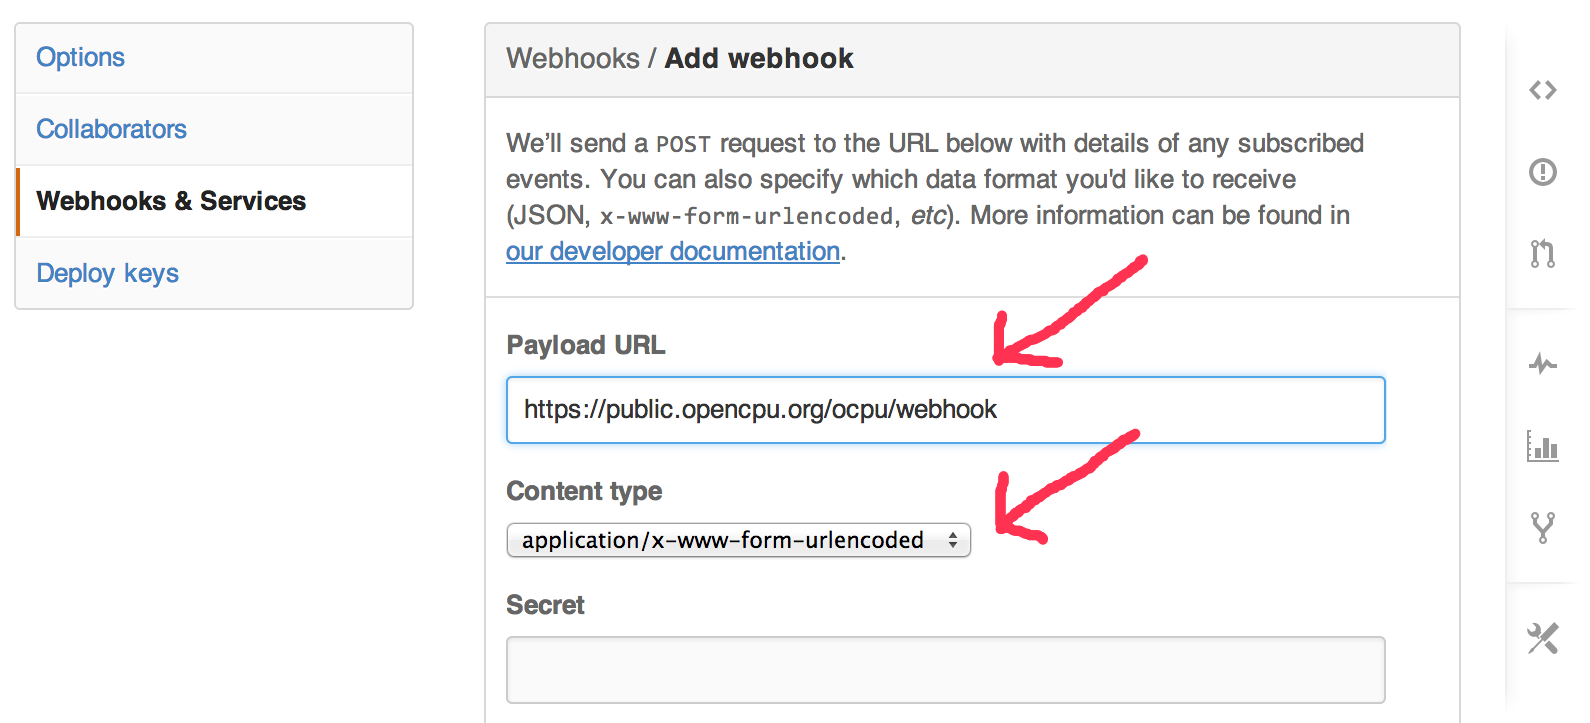
\includegraphics[scale=0.4]{grafics/githook.png}
    \caption{Nastavení webhook na~GitHub pro~umístění R balíčku na~veřejném serveru \cite{OpenCPUwebhook}}
\end{figure}

Single-user server vhodný pro~lokální spuštění OpenCPU aplikací je vlastně balíček R s~názvem \textit{opencpu}, lze tak jednoduše v~R nainstalovat příkazem:
\begin{verbatim}
install.packages("opencpu")
\end{verbatim}
Poté spustít příkazem:
\begin{verbatim}
library(opencpu)
\end{verbatim}
Pak je možné jednoduše načíst aplikaci z~GitHub pro~lokální použítí (k tomu je potřeba ještě balíček \textit{devtools}, který obsahuje funkci install\_github()), funkce opencpu\$browse("cesta\_k\_balíčku") otevře aplikaci ve výchozím prohlížeči.

\begin{alltt}
install_github("{uživatel}/{název_balíčku}")
opencpu\$browse("library/{název_balíčku}/www") 
\end{alltt}

Argument funkce opencpu\$browse je v~tomto případě cesta k~balíčku nainstalovaném v~jedné z~globálních knihoven na~serveru. Chceme-li tedy například nainstalovat a spustit lokálně v~prohlížeči OpenCPU aplikaci \textit{gitstats} z~veřejného repozitáře použijeme:

\begin{alltt}
install_github("opencpu/gitstats")
opencpu\$browse("library/gitstats/www") 
\end{alltt}

\begin{sloppypar}
Online pak tuto aplikaci najdeme na~adrese: \url{https://public.opencpu.org/ocpu/library/gitstats/www}.
\end{sloppypar}

\begin{sloppypar}
Aplikace konkrétních uživatelů na~účtu na~GitHub s~přidaným webhook jsou vždy na~adrese: \url{https://{uživatelské_jméno}.opencpu.org/{název_balíčku}/www}.
\end{sloppypar}

\subsection{Volání R funkcí z~webové stránky}

OpenCPU v~současné době používá jen HTTP metody GET a POST. GET se používá k~načítání zdrojů, tedy například k~načtení souboru nebo objektu, a POST k~RPC (Remote Procedure Call), tedy k~vzdálenému volání funkcí nebo spouštění skriptů. Požadavek POST je platný pouze s~cílovou URL skriptu nebo funkce. Seznam návratových stavových kódu OpenCPU, které by klient měl být schopen interpretovat je uveden na~adrese: \url{https://www.opencpu.org/api.html#api-status}.

\begin{sloppypar}
K testování je možné také použít tuto testovací stránku OpenCPU: \url{https://public.opencpu.org/ocpu/test/}. Nebo je možné z~příkazové řádky použít nástroj \textit{curl}, který slouží k~přenosu dat z/na server a jedním z~protokolů, které podporuje je také HTTP. Při použití metody POST, slouží k~přidání argumentů přepínač '-d'. Například k~volání funkce rnorm s~parametry n=10 a mean=5, z~balíčku stats (jedna z~oficiálních aplikací OpenCPU) použijeme:
\end{sloppypar}

\begin{alltt}
curl https://public.opencpu.org/ocpu/library/stats/R/rnorm -d
"n=10\&mean=5"
\end{alltt}

Pokud jde o~jiný, než veřejný server OpenCPU, nahradíme adresu veřejného serveru:

\begin{alltt}
https://\{adresa_serveru\}/ocpu/library/\{název_balíčku\}/
R/\{název_funkce\}
\end{alltt}
 
Kořenová složka /ocpu/ je výchozí nastavení serveru, jeho administrátor ho však může změnit.

Opět pokud jde o~balíček konkrétního uživatele na~veřejném serveru opencpu, bude URL:
\begin{alltt}
https://\{uživatelské_jméno\}.opencpu.org/
\{jméno_balíčku\}/R/\{název_funkce\}
\end{alltt}

Jako výstup testovaného volání funkce dostaneme: 
\begin{alltt}
/ocpu/tmp/x0a411c0928/R/.val
/ocpu/tmp/x0a411c0928/stdout
/ocpu/tmp/x0a411c0928/source
/ocpu/tmp/x0a411c0928/console
/ocpu/tmp/x0a411c0928/info
/ocpu/tmp/x0a411c0928/files/DESCRIPTION
\end{alltt}

Kde \uv{x0a411c0928} je ID relace. Relace je vlastně kontejner, který obsahuje prostředky vytvořené vzdáleným voláním funkce nebo skriptu. Například cesta url{https://public.opencpu.org/ocpu/tmp/x0a411c0928/R/.val/print} drží výstupní hodnoty funkce. Významy těch ostatních a vůbec všech možných cest, které můžete dostat jako návratovou hodnotu naleznete tady: \url{https://www.opencpu.org/api.html#api-session} a tady potom tabulku možných výstupních formátů: \url{https://www.opencpu.org/api.html#api-formats}.

Konkrétní kód, který bude volat funkci R z~balíčku se odvíjí od použitého programovacího jazyka.

Další možnost je k~volání funkcí R a k~zobrazování jejich výstupů na~stránce použít JavaScriptovou knihovnu opencpu.js, pak je nutné do hlavičky stránky zahrnout odkazy nejprve na~javascriptovou knihovnu jquery.js a poté na~knihovnu opencpu.js (je nutné dodržet toto pořadí). 
Je vhodné místo online odkazů na~knihovnu přidávat použitou aktuální verzi jako součást balíčku, protože je knihovna v~aktivním vývoji a aktuální verze se může čas od času radikálně změnit. Knihovna opencpu.js staví na~knihovně jQuery a umožňuje tak volat R funkce pomocí AJAXu (Asynchronous JavaScript and XML). Knihovna funguje ve všech moderních prohlížečích, a je primárně určena pro~vývoj aplikací. Úložiště veřejných OpenCPU aplikací je k~dispozici na~adrese \url{http://github.com/opencpu}. 

Doporučená struktura pro~OpenCPU aplikace je, aby byly webové stránky součástí balíčku R, podle konvence jsou tyto stránky umístěny v~balíčku v~podsložce /inst/www/. Díky tomu, že jsou stránky součástí balíčku, jsou aplikace snadno distribuovatelné a je možné je používat offline. Navíc to zajišťuje, že frontend aplikace a backend (kód R) jsou synchronizovány. Je zde ale také možnost použít tzv.CORS - Cross Domain OpenCPU Request, a tak použít knihovnu opencpu.js z~externího webu. V~tomto případě je nutné specifikovat adresu externího serveru OpenCPU pomocí ocpu.seturl():\cite{OpenCPUjsLibrary}
\begin{verbatim}
ocpu.seturl("//public.opencpu.org/ocpu/library/{název_balíčku}
/R").
\end{verbatim}

Knihovna implementuje dvě základní bezestavové funkce k~volání funkcí R, jednu pro~funkce generující grafy, druhou pro~funkce vracející nějaká data. Ty jsou snadno použitelné, protože berou přímo výstup z~funkce R a není zapotřebí žádná správa relací. Pomocí pluginu rplot můžeme zobrazovat grafy v~divu na~naší webové stránce:
\begin{alltt}
\$("#div_id").rplot(fun, [,args] [,callback])
\end{alltt}
Funkce vrací jqXHR jQuery objekt. Argument \textit{fun} obsahuje název funkce R, \textit{args} je pole parametrů R funkce a \textit{callback} je pro~callback funkci (funkci zpětného volání) a pro~zobrazení grafu v~divu na~stránce není potřeba, volá se jen pro~relační objekty. Tato funkce zobrazí graf na~webové stránce v~divu, jehož id je div\_id. Pro volání funkce R vracející data, využijeme funkci:
\begin{alltt}
ocpu.rpc(fun, [,args] [,complete])
\end{alltt}
Funkce opět vrací jqXHR jQuery objekt. Argumenty \textit{fun} a \textit{args} mají stejný význam jako u~předchozí funkce a argument \textit{complete} je opět callback funkce, volá se pouze v~případě úspěchu a má jeden argument, kterým je návratová hodnota funkce R. 

Tyto funkce dobře poslouží pro~aplikace pouze s~jedním voláním funkce R a jedním výstupem. Nicméně jiné aplikace mohou potřebovat sofistikovanější interakci s~R relací. Proto knihovna implementuje také funkce pro~správu relací. 

Relační ekvivalent k~funkci ocpu.rpc je funkce 
\begin{alltt}
ocpu.call(fun, [,args] [,callback])
\end{alltt}
Argumenty \textit{fun} a \textit{args} jsou stejné, rozdíl je pouze v~argumentu \textit{callback}, tento argument je JSON objekt osahující data vrácená R funkcí. Jde o~objekt relace. Objekt relace je třída Javascriptu, která obsahuje ID realce. Z~toho poté lze asynchronně získat data, grafy, soubory atd. Tento objekt může být také použít k~předání vrácené hodnoty R jako argument další funkci, aniž by objekt musel být načítán. V~opencpu.js existují 4 typy argumentů: základní JavaScript hodnota / objekt (automaticky převedeny do R přes JSON), objekt relace (představuje hodnotu R z~předchozího volání funkce), soubor a fragment kódu \cite{OpenCPUjsLibrary}. Seznam a popis dostupných metod nad relačními objekty lze najít tady: \url{https://www.opencpu.org/jslib.html#lib-session}. 

\chapter[Analýza: Sage]{Analýza Sage a možnosti jeho použití ve webové aplikaci - Sage Cell Server}
\section{Seznámení se Sage}
%kdo to vytvořil, proč
%obecný úvod

\textit{SageMath} (často zkráceně \textit{Sage}) je počítačový algebraický systém (CAS) sloužící hlavně pro~matematické výpočty a geometrické experimentování. Název je zkratkou z~anglického \textbf{S}oftware for \textbf{A}lgebra and \textbf{G}eometry \textbf{E}xperimentation. Tento software je Open Source vydaný pod licencí GNU \cite{SageIntro}. Je multiplatformní, dostupný pro~Linux, Mac OS X a díky virtualizaci také pro~Windows. První verze byla odhalena v~únoru 2005 \cite{FoCM2011}. Zakladatelem a vedoucí osobností celého projektu je William Stein z~University of Washington, Seattle, Washington, USA.

Hlavním cílem projektu \textit{Sage} je vytvořit životaschopnou Open Source alternativu k~placeným algebraickým systémům Magma, Maple, Mathematica a MATLAB. Narozdíl od těchto systémů má však Sage všechny zdrojové kódy včetně historie úprav volně k~dispozici \cite{tracSage}. V~Sage developer trac může také kdokoliv nahlásit objevené chyby v~systému, nebo se podílet na~jeho vývoji. Sage tak kolem sebe od roku 2005 vytvořil silnou uživatelskou komunitu, jenž dále tento systém rozvíjí. Vyvojáři však musí respektovat, že je Sage zveřejněn pod licencí GNU (chtějí-li tak své úpravy a nadstavby systému dále šířit, musí je šířit také pod touto licencí).  

\textit{Sage} používá programovací jazyk Python, ale obsahuje také kompilátory jazyka C/C++ a používá jazyk \textit{Cython}. \textit{Cython} je upravená verze Pythonu, která je před interpretací převedena na~kód v~jazyce C a posléze kompilátorem jazyka C zkompilována. To je užitečné zejména ke složitějším matematickým výpočtům, protože jazyk \textit{Cython} je výrazně rychlejší, než jazyk Python \cite{Cython}.

Sage je možné používat ve dvou rozhraních - konzolovém, nebo webovém. Konzolové rozhraní je vhodné ke kratším výpočtům nebo ke spouštění externích skriptů. Webové rozhraní se spouští z~konzolového rozhraní příkazem \texttt{notebook()}. Zde pak uživatel pracuje s~tzv. \textit{worksheety}. Vlastní GUI Sage nemá, je však možné použít online cloud \cite{SageCloud}.  Zde má uživatel po registraci, která je zdarma, možnost spravovat své projekty, případně je sdílet s~jinými uživateli. Toto online rozhraní pro~Sage také usnadňuje uživateli práci, protože mu umožňuje vkládání předdefinovaných funkcí a grafů.

Sage poskytuje rozhraní také pro~jiné algebraické systémy a umožňuje tak spouštět funkce mnoha systémů z~jednoho konzolového rozhraní. Tyto systémy však musí mít uživatel nainstalované. Instalační balíček Sage zahrnuje např. balíčky GAP, PARI, Singular, Maxima a také R. Nezahrnuje však balíčky jako např. Octave, a také placené systémy MAGMA, Maple a Mathematica \cite{SageInterfaces}. Použití těchto systémů z~rozhraní Sage, obzvlášť z~toho konzolového, ale nemusí být tak komfortní, jak jsou uživatelé zvyklí. Pracuje-li uživatel ve worksheetu webového rozhraní, je možné zde specifikovat jazyk, v~kterém má být interpretován. Toto nastavení se ale týká celého worksheetu, není tedy možné dvě jeho různé buňky interpretovat odlišně. 

Velkou předností Sage je schopnost vytvářet interaktivní demonstrace. To je možné díky příkazu \texttt{interact}, který je součástí Sage od roku 2008. Ten umožňuje vkládat do buňky Sage textová pole, posuvníky, tlačítka a rozbalovací menu. Archiv aplikací vytvořených komunitou Sage Interact je k~dispozici online \cite{SageInteract}. 

Integraci \textit{Sage} do webové aplikace je možné provézt díky projektu \textit{Sage Cell Server}, jeho první verze vyšla v~lednu 2011 \cite{SageCellServer}. 


\section{Statistické výpočty v~Sage}
%z hlediska statistiky
%tzn. grafy, knihovna R,...
%interact
\textit{Sage} používá syntaxi jazyka Python a je tak možné použít všechny jeho dostupné knihovny. Zároveň může Sage využívat knihovny napsané pro~jazyk C/C++. Python je interpretovaný jazyk. Díky tomu je jednoduchý pro~implementaci a ladění, ale jeho kód může být pomalejší. To je jeden z~důvodů, proč Sage využívá ještě vlastní modifikaci jazyka Python, \textit{Cython} \cite{CodingCython}. Cython obsahuje oproti jazyku Python některá rozšíření a umožňuje tak v~Sage vysokoúrovňové, objektově orientované, funkcionální a dynamické programování. Kód tohoto jazyka může vypadat jako kód jazyka Python, je ale nejprve přeložen na~optimalizovaný kód jazyka C/C++ a poté zkompilován. Díky tomu je jazyk Cython dobře znám vyvojářům v~Pythonu, ale má potenciál být mnohem rychlejší. 

Příkaz \texttt{interact} nám v~aplikaci umožňuje využít interaktivní prvky pro~nastavení proměnných uživatelem a následné překreslování výsledků. Pro použití příkazu je nutné vytvořit třídu, které v~parametrech konstruktoru předáme informace o~proměnných, jejichž hodnoty se budou měnit pomocí ovládacích prvků. Při každé změně hodnoty se vykoná celý kód za příkazem interact. Jednoduše lze použít příkaz interact například pro~výpočet faktoriálu, kde uživatel volí hodnotu $x$ z~množiny $\left \{0,1,2,3,4,5 \right \}$ (obrázek 2.1). Kód pro~použití příkazu interact pro~výpočet $f(x)=x!$, kde $x\in\left \{0,1,2,3,4,5 \right \}$ vypadá následovně:

\begin{verbatim}
@interact
def factorial(n=(0..5)):
   return 1 if n == 0 else n * factorial(n - 1)
\end{verbatim}

\begin{figure}[ht]
    \centering
    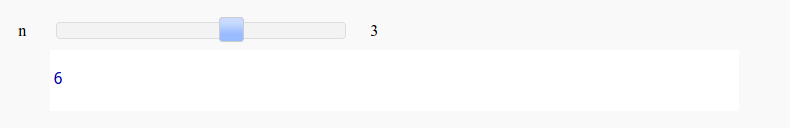
\includegraphics[scale=0.4]{grafics/factorial.png}
    \caption{Jednoduché použití příkazu \texttt{interact} pro~výpočet faktoriálu.}
\end{figure}

Čistý jazyk Python, podobně jako jiné programovací jazyky, obsahuje základní matematické funkce a operátory. Pro složitější výpočty v~Pythonu je pak nutné zvolit některé z~jeho knihoven. Python nabízí mnoho knihoven poskytující funkce vhodné pro~statistické výpočty:

\begin{description}

\item[random] Pseudo-náhodné číselné generátory pro~různá rozdělení \cite{random}.

\item[statistics] \begin{sloppypar}Obsahuje funkce pro~statistické výpočty nad reálnými číselnými daty. Jde však pouze o~několik základních funkcí jako výberový průměr a rozptyl \cite{statistics}.\end{sloppypar}

\item[Numpy, Matplotlib, SciPy, IPython, pandas] \begin{sloppypar}Tyto nástroje jsou součástí tzv. \textit{SciPy Stack} kolekce open source softwarů pro~vědecké výpočty v~Pythonu \cite{SciPy}. \textit{Numpy} je základní balíček pro~numerické výpočty. Definuje numerické pole, maticové typy a základní operace mezi nimi \cite{NumPy}. \textit{Matplotlib} je balíček pro~vykreslovaní jak 2D, tak 3D grafů \cite{matplotlib}. Knihovna \textit{SciPy} je sbírka numerických algoritmů a doménově specifických nástrojů, včetně nástrojů pro~optimalizaci, statistiku a mnoho dalšího \cite{SciPy}. Interaktivní rozhraní \textit{IPython} umožňuje uživateli zpracovávat data a testovat hypotézy \cite{IPython}.  \textit{Pandas} poskytuje vysoce výkonné a snadno použitelné datové struktury \cite{pandas}. \end{sloppypar}

\item[rpy2] \begin{sloppypar} \textit{Rpy} poskytuje nízkoúrovňové rozhraní pro~R v~Pythonu. \textit{Rpy2} je jeho přepracovaná nová verze. Poskytuje rozhraní vyšší úrovně, je tak možné volat funkce z~grafických balíčků a používat struktury a funkce R \cite{rpy2}. \end{sloppypar}

\item[python-statlib] \begin{sloppypar} Balíček \textit{python-statlib} \cite{statlib} kombinuje tři statistické moduly pro~Python: \textit{stats} (kolekce základních statistických funkcí pro~Python \cite{StatsDoc}), \textit{pstats} (poskytuje užitečné nástroje pro~manipulaci s~listy a polemi \cite{PstatDoc}) a \textit{matfunc} (modul pro~matematické operace nad vektory, tabulkami a maticemi \cite{Matfunc}).\end{sloppypar}

\item[statsmodels] \begin{sloppypar} Modul umožňující uživateli zkoumat data, odhadovat statistické modely a provádět statistické testy \cite{statsmodels}. \end{sloppypar}

\item[PyMC] \begin{sloppypar} Model realizující Bayesovské statistické modely a stochastické metody používající pseudonáhodná čísla (např. Monte Carlo). Je flexibilní a rozšiřitelný, díky čemuž je použitelný pro~velkou sadu problémů \cite{PyMC}. \end{sloppypar}

\item[PyMix] \begin{sloppypar} Knihovna poskytující funkce pro~aplikace zpracovávající data. Poskytuje konečné modely pro~diskrétní i spojité funkce, širokou škálu rozdělení (normální, exponenciální, diskrétní,...), Bayesovské modely, parametrové odhady a další \cite{PyMix}.\end{sloppypar}

\end{description}

Druhou možností, jak v~Sage provádět statistické výpočty, je zvolit jiný programovací jazyk, který snadno umožňuje rozsáhlou škálu statistických výpočtů a který Sage umí interpretovat. Ideální je vybrat jazyk, který je k~dispozici již se základní instalací Sage, tedy jazyk R. Implementace statistických výpočtů se tak pro~uživatele zjednodušuje, ale zároveň přichází o~výhodu Sage, příkaz \texttt{interact}. V~případě použití ve webové aplikaci však lze vlastnosti interaktivních Sage aplikací snadno nahradit použítím JavaScriptu.

\section{Sage Cell Server}

\textit{Sage Cell Server} je open-source webové rozhraní pro~\textit{Sage}. Kromě toho také může být použit k~vložení \textit{Sage} do libovolné webové stránky. Jedna vložená buňka Sage Cell Server pak odpovídá jedné buňce ve webovém rozhraní.

K samotným výpočtům můžeme využít vlastní (zdrojové kódy k~instalaci jsou k~dispozici na~GitHub \cite{sagemathGithub}), nebo veřejný server poskytovaný tímto projektem. 

Vložení \textit{Sage} do stránky pak probíhá jednoduše ve dvou krocích: 

\begin{enumerate} 
  \item Do hlavičky HTML stránky uživatel vloží následující kód: 
  
\begin{alltt}
<script src="https://sagecell.sagemath.org/static/
jquery.min.js">
</script>
<script src="https://sagecell.sagemath.org/static/
embedded\_sagecell.js">
</script>
<script>
sagecell.makeSagecell({"inputLocation": ".sage"});
</script>
\end{alltt}

Adresa sagecell.sagemath.org může být případně nahrazena adresou serveru uživatele, na~kterém je nainstalována služba \textit{SageCell}. První dva tagy <skript> slouží k~načtení Javascriptové knihovny jquery.js a skriptu \textit{SageCell} do webové stránky, třetí pak k~převedení všech HTML elementů s~třídou \textit{sage} na~buňku \textit{SageCell}.

Pokud uživatel do stránky vkládá mnoho stylů (jde-li například o~blog nebo deck.js prezentaci), může nastat konflikt mezi stylem stránky a stylem \textit{SageCell}, pak je možné pod tyto tagy připojit ještě jeden, který načte speciální styly pro~\textit{SageCell} objekty:

\begin{alltt}
<link rel="stylesheet" type="text/css" 
href="https://sagecell.sagemath.org/static
/sagecell_embed.css">
\end{alltt}

  \item Poté je třeba vložit kód do těla stránky. Kód je obalen do tagů <script>, díky čemuž není interpretován jako kód HTML. 

\begin{alltt}
<div class="sage">
  <script type="text/x-sage">kód_Sage</script>
</div>
\end{alltt}
  
\end{enumerate}

Při vkládání \textit{Sage} modulů lze upravit nastavení buněk. Je možné nastavit v~jakém jazyce budou buňky interpretovány. Uživatel může upravit popis potvrzovacího tlačítka, nebo ho úplně skrýt, stejně jako další části modulu. 

\chapter{Vybrané statistické metody}

\textit{Matematická statistika} jako vědecká disciplína zkoumá, zpracovává a vyhodnocuje data. Provádí experimenty, jejichž cílem je zjistit data o~dané populaci (soubor jakýchkoliv prvků, které budeme zkoumat). Narozdíl od teorie pravděpodobnosti, která na~základě znalostí chování určité náhodné veličiny určuje pravděpodobnost určitého výsledku, matematická statistika na~základě dat hledá vlastnosti náhodné veličiny. V~testovací aplikaci data dostaneme zadána uživatelem. Aplikace pak tato data analyzuje. V~této kapitole se proto budeme zabývat především analýzou náhodných veličin. Definice a věty jsou čerpány ze skript pana Jiřího Anděla \cite{Anděl}, ze skript Aplikovaná statistika pana Jiřího Pavlíka \cite{VŠCHT} a z~knihy Graphical methods for data analysis Johna M. Chamberse \cite{GraphMethods}.

\section{Základní pojmy teorie pravděpodobnosti}
Pokud není výsledek nějakého pokusu nebo děje jednoznačně určen podmínkami, za nichž se odehrává, můžeme různě možné výsledky považovat za \textit{elementární jevy}. Ty budeme v~tomto textu značit $\omega$, množinu všech elemntárních jevů, nazývaný táké \textit{prostor elementárních jevů}, pak $\Omega$. Nechť je na~prostoru $\Omega$ dána nějaká $\sigma$-algebra $\mathcal{A}$ jeho podmnožin. Tyto podmnožiny se nazývají \textit{náhodné jevy}. Právě jednotlivým množinám patřícím do $\mathcal{A}$ se pak připisuje pravděpodobnost pomocí nějaké pravděpodobnostní míry $\mathtt{P}$. Trojice $(\Omega,\mathcal{A},\mathtt{P})$ se nazývá \textit{pravděpodobnostní prostor}.

Nechť $\mathbb{R}$ je reálná přímka a $\mathcal{B}$ systém borelovských podmnožin. Nechť $X(\omega)$ je měřitelná funkce z~$(\Omega,\mathcal{A},\mathtt{P})$ do $(\mathbb{R},\mathcal{B})$. Pak se $X(\omega)$ nazývá \textit{náhodná veličina} a značí se $X$. Každé borelovské množině $B\in\mathcal{B}$ lze přiřadit její vzor $X^{-1}(B) = \left \{\omega \in \Omega : X(\omega)\in B \right \}$ a pravděpodobnostní míru $Q(B) = \mathtt{P}{X^{-1}(B)}$~\cite{Anděl}. \textit{Indukovanou míru} $Q$ nebo také \textit{zákon rozdělení náhodné veličiny X} budeme obvykle nazývat stručně \textit{rozdělení X}.

Položíme-li $B=(-\infty, x \rangle$, dostaneme 
$$F(x) = \mathtt{P}{(X\leq x)}.$$
Této funkci $F$ říkáme \textit{distribuční funkce} a její hodnoty jednoznačně určují rozdělení $X$.

Distribuční funkce $F$ náhodné veličiny má následující vlastnosti: je neklesající, zleva spojitá a platí, že $\lim_{x\rightarrow-\infty} F(x) =0$ a $\lim_{x\rightarrow\infty} F(x) =1$. Tato funkce může mít nejvýše spočetně mnoho bodů nespojitosti.

V teorii pravděpodobnosti mluvíme o~dvou druzích distribuční funkce:

\begin{enumerate}[(a)]
\item Je-li distribuční funkce $F$ po částech konstantní, pak jde o~\textit{diskrétní rozdělení}.

\item Existuje-li taková funkce $f(x)$, že platí
$$F(x) =  \int_{-\infty}^{x}f(t)dt,$$
pak mluvíme o~\textit{spojitém rozdělení}. Funkce $F(x)$ se v~takovém případě nazývá hustota pravděpodobnosti náhodné veličiny $X$.
\end{enumerate}

Pro integrály náhodných veličin se ve statistice používá symbol $\mathtt{E}$ (expectation) \cite{Anděl}. $\mathtt{E}X = \int_R x dQ(x)$, kde $Q$ je rozdělení náhodné veličiny $X$. Pro diskrétní náhodnou veličinu $X$ dostáváme $\mathtt{E}X = \sum_i x_i \mathtt{P}(X=x_i)$. Pro spojitou náhodnou veličinu $X$ s~hustotou pravděpodobnosti $f(x)$ dostáváme $\mathtt{E}X = \int_R x f(x) dx$. $X(\omega)d\mathtt{P}(\omega)$ je \textit{střední hodnota}, pokud tento integrál existuje. Obvykle se provádí konkrétní výpočet $\mathtt{E}X=\int{\mathbb{R}} xdF(x)$, protože většinou známe pouze distribuční funkci. Pokud $a$ je nějaká konstanta, pak $\mathtt{E}a=a$. 

Označme ${\mu}'_{k}=\mathtt{E}X^k, k=1,2,...$. Číslo ${\mu}'_{k}$ se nazývá \textit{obecný moment k}-tého řádu. Existuje-li moment ${\mu}'_{1}$ a je-li konečný, pak definujeme $\mu_{k}=\mathtt{E}(X-\mathtt{E}X)^k, k=0,1,...$. Číslo $\mu_{k}$ se nazývá \textit{centrální moment k}-tého řádu \cite{Anděl}. Nejdůležitější centrální moment je $\mu_{2}$, který se nazývá \textit{rozptyl} a obvykle se značí $\sigma^2$, někdy ho ale budeme značit $\var X$. \textit{Směrodatná odchylka} $\sigma$ je definována $\sigma=\sqrt{\var X}$ a platí, že $\sigma\geq 0$. Po úpravě dostáváme, že $\sigma^2 = \mathtt{E}X^2 - (\mathtt{E}X)^2$. Dále platí, že pokud jsou $a$ a $b$ reálná čísla a existuje-li $\mathtt{E}X$, pak $\mathtt{E}(a+bX)=a+b\mathtt{E}X$. Pokud $\mathtt{E}X^2<\infty$, pak $\var(a+bX)=b^2\var X$. Pro náhodné veličiny X a Y s~konečnou střední hodnotou platí $\mathtt{E}(aX+bY)=a\mathtt{E}X+b\mathtt{E}Y$. Kromě střední hodnoty jsou důležitými charakteristikami \textit{kvantily}. 100p\%-ním kvantilem spojité náhodné veličiny $X$ (přičemž pro~$p$ platí, že $0<p<1$) nazveme číslo $u_{p}$ takové, že

$$\mathtt{P}(X\leq u_{p})=p \mbox{ neboli } F(u_{p})=p,$$

kde $F(x)$ je distribuční funkce veličiny $X$. 50\% kvantil nazýváme \textit{medián}.

\subsection{Kovariance a korelace}
Kromě číselných charakteristik jednotlivých náhodných veličin $X$ a $Y$ jsou důležité číselné charakteristiky, které vyjadřují jejich vzájemnou souvislost.

Mějme náhodné veličiny $X$ a $Y$ s~konečnými druhými momenty. Pak definujeme \textit{kovarianci} náhodných veličin $X$ a $Y$ vztahem

$$\cov(X,Y)=\mathtt{E}\left[ (X-\mathtt{E}X)(Y-\mathtt{E}Y) \right ].$$

A (Pearsonův) \textit{korelační koeficient}

$$\varrho(X,Y)=\frac{\cov(X,Y)}{\sqrt{\var X}\sqrt{\var Y}}$$


\section{Vybraná spojitá rozdělení}
Zde uvedeme příklady normálního, exponenciálního a rovnoměrného rozdělení spolu s~jejich základními charakteristikami - střední hodnotou a rozptylem.


\subsection{Normální rozdělení}
Nechť $\mu\in\mathbb{R}$ a $\sigma>0$ jsou dané konstanty (parametry). \textit{Normální rozdělení} (nebo také \textit{Gaussovo}) je určeno hustotou

$$f(x)=\frac{1}{\sqrt{2\pi}\sigma}e^{-\frac{(x-\mu)^2}{2\sigma^2} }, \mbox{ pro~} x\in(-\infty,+\infty).$$

a označuje se symbolem $N \sim (\mu,\sigma^2)$.

Střední hodnota $\mathtt{E}X$ a rozptyl $\var X$ náhodné veličiny s~normálním rozdělením jsou rovna:

$$\mathtt{E}X = \mu,$$
$$\var X=\sigma^2.$$ 

\subsection{Exponenciální rozdělení}
Nechť $\lambda > 0$. \textit{Exponenciální rozdělení} $Exp(\lambda)$ má hustotu
$$
f(x) = \left\{ \begin{array}{rl}
\lambda e^{-\lambda x} &\mbox{ pro~$x>0$,} \\
0 &\mbox{ jinde.}
\end{array} \right.
$$

Střední hodnota a rozptyl náhodné veličiny s~exponenciálním rozdělením: 

$$\mathtt{E}X=\frac{1}{\lambda},$$

$$\var X = \frac{1}{\lambda^2}.$$


%citace z~přednášek????

\subsection{Rovnoměrné rozdělení}
Nechť $(a,b)$ je konečný nedegenerovaný interval, kde $a<b, a,b\in\mathbb{R}$. \textit{Rovnoměrné rozdělení} $U(a,b)$ má hustotu

$$
f(x) = \left\{ \begin{array}{rl}
\frac{1}{b-a} &\mbox{ pro~$x\in\left \langle a,b  \right \rangle$,} \\
0 &\mbox{ jinde.}
\end{array} \right.
$$

a platí pro~něj
$$\mathtt{E}X=\frac{a+b}{2},$$

$$\var X=\frac{(b-a)^2}{12}.$$


\section{Bodové odhady}


Nechť $X_{1},...,X_{n}$ je posloupnost nezávislých stejně rozdělených náhodných veličin s~rozdělením $Q$. Pak říkáme, že $X_{1},...,X_{n}$ je \textit{náhodný výběr} z~rozdělení $Q$. Číslo $n$ se nazývá \textit{rozsah výběru}. 

Nechť $\mathbf{X}={(X_{1},\dotsc,X_{n})}$ má hustotu $f(x,\boldsymbol{\theta})$, kde $\boldsymbol{\theta} = (\theta_1,\dotsc,\theta_m)$ je neznámý $m$-rozměrný parametr. Na~základě vektoru $\mathbf{X}$ je třeba získat pokud možno co nejlepší odhad parametru $\boldsymbol{\theta}$, o~kterém je předem známo pouze tolik, že patří do nějakého parametrického prostoru $\Omega \subset \mathbb{R}^{m}$. Jde-li nám o~\textit{bodový odhad}, hledáme nějaké měřitelné zobrazení $g:(\mathbb{R}^{n},\mathcal{B})\rightarrow (\mathbb{R}^{m},\mathcal{B}_{m})$ tak, aby náhodný vektor $\hat{\boldsymbol{\theta}} = g(\mathbf{X})$ v~nějakém rozumném smyslu co nejlépe aproximoval hodnotu $\boldsymbol{\theta}$.

\subsection{Vlastnosti odhadu} 
Řekneme, že odhad $\hat{\boldsymbol{\theta}}$ parametru $\boldsymbol{\theta}$ je \textit{nestranný}, platí-li $\mathtt{E}\mathbf{T}=\boldsymbol{\theta}$ pro~každé $\boldsymbol{\theta}\in\Omega$. Platí-li $\mathtt{E}\mathbf{T}=\boldsymbol{\theta} + \mathbf{b}(\boldsymbol{\theta})$, kde funkce $\mathbf{b}$ není identicky rovna nule na~množině $\Omega$, nazývá se odhad $\hat{\boldsymbol{\theta}}$ \textit{vychýlený}. Vektoru $\mathbf{b}(\boldsymbol{\theta})$ se pak říká \textit{vychýlení odhadu} $\mathbf{T}$ v~bodě $\boldsymbol{\theta}$. 
Obvykle se snažíme, aby byl odhad také nestranný a konzistentní. Pro definici těchto pojmů odkazujeme čtenáře na~\cite[p.101-102]{Anděl}. 

\subsection{Střední hodnota, rozptyl, směrodatná odchylka a medián}

Mezi nejužívanější bodové odhady patří odhady střední hodnoty, rozptylu a směrodatné odchylky.

Položme

$$\bar{X}=\frac{1}{n}\sum_{i=1}^{n}X_{i} \quad \text{a} \quad S^{2}=\frac{1}{n-1}\sum_{i=1}^{n}(X_{i}-\bar{X})^2.$$

Veličina $\bar{X}$ se nazývá \textit{výběrový průměr} (bodový odhad střední hodnoty) a veličina $S^{2}$ \textit{výběrový rozptyl} (bodový odhad rozptylu). Hodnotu $\sqrt{S^{2}}$ nazýváme \textit{výběrová směrodatná odchylka} (bodový odhad směrodatné odchylky). Základním bodovým odhadem \textit{mediánu $\tilde{x}$} pro~náhodný výběr pro~liché $n$: $x_{((n+1)/2)}$, pro~sudé $n$ pak: $(x_{(n/2)}+x_{((n/2)+1)})/2$.


\subsection{Metoda maximální věrohodnosti}
Jednou z~metod získávání velmi dobrých odhadů je \textit{metoda maximální verohodnosti}. Jejím cílem je maximalizovat věrohodnostní funkci pro~dané naměřené hodnoty. 

Mějme náhodný výběr $X_{1},...,X_{n}$ jehož sdružené rozdělení je určeno pomocí: 

$$f(\boldsymbol{x},\boldsymbol{\theta}(x_i)) = \prod_{i=1}^{n}f(x_{i})
\mbox{ pro~spojité rozdělení, resp.}$$

$$p(\boldsymbol{x},\boldsymbol{\theta}(x_i)) = \prod_{i=1}^{n}\mathtt{P}(X_{i}=x_{i})
\mbox{ pro~diskrétní rozdělení,}$$

\noindent kde $\boldsymbol{\theta}\in\Omega$. Při pevné hodnotě $\boldsymbol{x}$ se funkce $f(\boldsymbol{x},\boldsymbol{\theta}(x_i))$, resp. $p(\boldsymbol{x},\boldsymbol{\theta}(x_i))$ jakožto funkce $\boldsymbol{\theta}$ nazývá \textit{věrohodnostní funkce} a značí se $L(\theta,\boldsymbol{x})$.

\begin{sloppypar}
Hodnota $\hat{\boldsymbol{\theta}}$ parametru $\boldsymbol{\theta}$, která maximalizuje věrohodnostní funkci $f(\boldsymbol{x},\boldsymbol{\theta}(x_i))$, resp. $p(\boldsymbol{x},\boldsymbol{\theta}(x_i))$ pro~dané $\boldsymbol{x}$, se nazývá \textit{maximálně věrohodný odhad} (MLE) parametru $\boldsymbol{\theta}$.\end{sloppypar}

Funkce $l(\boldsymbol{\theta},\boldsymbol{x})=\ln f(\boldsymbol{x},\boldsymbol{\theta}(x_i))$, resp. $l(\boldsymbol{\theta},\boldsymbol{x})=\ln p(\boldsymbol{x},\boldsymbol{\theta}(x_i))$ se jakožto funkce proměnné $\boldsymbol{\theta}$ při pevném $\boldsymbol{x}$ nazývá \textit{logaritmická věrohodnostní funkce}. Často se vyplatí maximalizovat funkci $l(\boldsymbol{\theta},\boldsymbol{x})$, protože tak v~rovnici dostaneme sumu za produkt. Přičemž maxima obou funkcí jsou stejná.

Nyní provedeme odhad parametrů spojitých rozdělení normálního, exponenciálního a rovnoměrného, pomocí metody maximální věrohodnosti.

\subsubsection{Normální rozdělení}
Nechť $X_1,\dotsc,X_n$ je náhodný výběr z~normálního rozdělení $X \sim N(\mu, \sigma^2)$

V tomto případě je výhodné maximalizovat logaritmickou věrohodnostní funkci

\begin{align*}
l(\mu,\sigma^2,\boldsymbol{x}) 
& = \ln(L(\mu,\sigma^2,\boldsymbol{x}))\\
& = \ln((2\pi \sigma^2)^{-n/2}e^{-\frac{1}{2\sigma^2}\sum^{n}_{j=1}(x_j-\mu)^2})).\\
\end{align*}


\noindent O~maximu můžeme říct, že pro~něj platí

$$\frac{\partial }{\partial \mu}l(\mu,\sigma^2,\boldsymbol{x}) = 0,$$

$$\frac{\partial }{\partial \sigma^2}l(\mu,\sigma^2,\boldsymbol{x}) = 0.$$

\noindent Parciální derivaci podle střední hodnoty upravujeme

\begin{align*}
\frac{\partial }{\partial \mu}l(\mu,\sigma^2,\boldsymbol{x}) \\
&=\frac{\partial }{\partial \mu}
(-\frac{n}{2}\ln(2\pi)-\frac{n}{2}\ln(\sigma^2)-\frac{1}{2\sigma^2}
\sum^{n}_{j=1}(x_{j}-\mu)^2) \\
&=\frac{1}{\sigma^2}\sum^{n}_{j=1}(x_{j}-\mu) \\
&=\frac{1}{\sigma^2}(\sum^{n}_{j=1}x_{j}-n\mu).\\
\end{align*}
\noindent A to je rovno nule jen když platí, že

$$\sum^{n}_{j=1}x_{j}-n\mu = 0.$$

\noindent Z~první podmínky pro~maximum tedy dostáváme maximálně věrohodný odhad~$\hat{\mu}$

$$\hat{\mu}=\frac{1}{n}\sum^n_{j=1}x_{j}=\bar{X}.$$

\noindent Parciální derivace podle rozptylu
\begin{align*}
\frac{\partial }{\partial \sigma^2}l(\mu,\sigma^2,\boldsymbol{x})\\
&=\frac{\partial }{\partial \sigma^2}
(-\frac{n}{2}\ln(2\pi)-\frac{n}{2}\ln(\sigma^2)-\frac{1}{2\sigma^2}
\sum^{n}_{j=1}(x_{j}-\mu)^2)\\
&= -\frac{n}{2\sigma^2}- \left [ \frac{1}{2}\sum^{n}_{j=1}(x_{j}-\mu)^2 \right ] \frac{d}{d \sigma^2} \left (\frac{1}{\sigma^2} \right )\\
&= -\frac{n}{2\sigma^2}- \left [ \frac{1}{2}\sum^{n}_{j=1}(x_{j}-\mu)^2 \right ] \left (- \frac{1}{(\sigma^2)^2} \right )\\
&=-\frac{n}{2\sigma^2}+
\left [ \frac{1}{2}\sum^{n}_{j=1}(x_{j}-\mu)^2 \right ]
\frac{1}{(\sigma^2)^2}\\
&=\frac{1}{2\sigma^2}
\left [ \frac{1}{\sigma^2}\sum^{n}_{j=1}(x_{j}-\mu)^2-n \right ]
\frac{1}{(\sigma^2)^2}.\\
\end{align*}
\noindent Musí platit, že $\sigma^2\neq0$, pak se tento výraz rovná nule jen když

$$\sigma^2=\frac{1}{n}\sum^{n}_{j=1}(x_{j}-\mu)^2.$$

\noindent Dostáváme tedy maximálně věrohodný odhad~$\hat{\sigma^2}$

$$\hat{\sigma^2}=\frac{1}{n}\sum^{n}_{j=1}(x_{j}-\hat{\mu})^2.$$

\subsubsection{Exponencíální rozdělení}
Nechť $X_1,\dotsc,X_n$ je náhodný výběr z~exponenciálního rozdělení $X \sim Exp(\lambda)$ 

V tomto případě je opět výhodnější maximalizovat logaritmickou věrohodnostní funkci

\begin{align*}
l(\lambda,\boldsymbol{x}) 
& = \ln(L(\lambda,\boldsymbol{x})) \\
& = \ln (\lambda^n e^{-\lambda \sum^{n}_{j=1}x_{j}}) \\
\end{align*}


\noindent Pro maximum platí

$$\frac{d}{d\lambda}l(\lambda,\boldsymbol{x})=0.$$

\noindent Zderivováním logaritmické věrohodnostní funkce získáváme

$$\frac{d}{d\lambda}l(\lambda,\boldsymbol{x})=\frac{d}{d\lambda}l(n\ln(\lambda)-\lambda\sum^{n}_{j=1}x_{j})=\frac{n}{\lambda}-\sum^{n}_{j=1}x_{j}.$$

\noindent Položíme rovné nule a dostáváme maximálně věrohodný odhad parametru~$\lambda$

$$\hat{\lambda}=\frac{n}{\sum^{n}_{j=1}x_{j}}=\frac{1}{\bar{X}}.$$

\subsubsection{Rovnoměrné rozdělení}
Nechť $X_1,\dotsc,X_n$ je náhodný výběr z~rovnoměrného rozdělení $X \sim U(a, b)$

Upravíme věrohodnostní funkci 

\begin{align*}
L(a,b,\boldsymbol{x}) 
&= \prod_{j=1}^{n}f(x_{j}) \\
&= \prod_{j=1}^{n}\frac{1}{b-a} \chi_{\left \langle a,b \right \rangle}(x) \\
&= \frac{1}{(b-a)^{n}}\prod_{j=1}^{n}\chi_{\left \langle a,b \right \rangle}(x) \\
\end{align*}

\noindent kde $\chi_{\left \langle a,b \right \rangle}(x)$ je charakteristická funkce množiny hodnot z~intervalu $\left \langle a,b \right \rangle$. Celý výraz $\prod_{j=1}^{n}\chi_{\left \langle a,b \right \rangle}(x)$ může nabývat pouze hodnoty $0$ nebo $1$. Hodnoty $1$ nabyde v~případě, že pro~všechna $x_{j}$ z~$x_{1},...,x_{n}$ platí, že jsou z~intervalu $\left \langle a,b \right \rangle$. V~případě, že $\exists x_{j} \notin \left \langle a,b \right \rangle$, pak celý výraz nabývá hodnoty $0$. Funkce nabývá vždy nezáporných hodnot, protože $a<b$, proto chceme-li najít maximum, musí výraz $\prod_{j=1}^{n}\chi_{\left \langle a,b \right \rangle}(x)=1$, z~čehož plyne, že $a\leq \min{x_{j}}_{j} < \max{x_{j}}_{j} \leq b$. Nyní tedy hledáme maximum výrazu $\frac{1}{(b-a)^n}$ takové, aby platil předchozí interval. Aby tento zlomek nabýval co nejvyšších hodnot, musí jmenovatel být co nejmenší, pak tedy musí být rozdíl $b-a$ co nejmenší, zároveň však musí být $a\leq\min{x_{j}}_{j}$ a $b\geq\max{x_{j}}_{j}$. Z~toho plyne, že maximálně věrohodný odhad parametrů $a$ a $b$ je 

$$\hat{a}=\min{X}, \hat{b}=\max{X}$$



\section{Odhady tvaru rozdělení}

\subsection{Histogram}
\textit{Histogram} je graf znázorňující, jak jsou četnosti rozděleny mezi zvolené intervaly hodnot zkoumané veličiny. Graf je rozdělen do tříd (intervalů), každé třídě vždy odpovídá jeden sloupec grafu. Šířka sloupce odpovídá velikosti intervalu a jeho výška četnosti hodnot v~tomto intervalu. Díky histogramu můžeme odhadovat tvar rozdělení. Tvar rozdělení můžeme dobře odhadnout také pomocí grafu empirické distribuční funkce (CDF).

\subsection{Empirická distribuční funkce}
Nechť $X_{1},...,X{n}$ je náhodný výběr z~rozdělení, které má distribuční funkci $F$. Budiž $x$ dané reálné číslo. Zaveďme náhodné veličiny

$$
\xi_{i}(x) = \left\{ \begin{array}{rl}
1 &\mbox{, je-li $X_{i}<x$,} \\
0 &\mbox{, je-li $X_{i}\geq x$.}
\end{array} \right.
$$

\noindent pro~$i=1,...,m$. \textit{Empirická distribuční funkce} je pro~každé $x \in \mathbb{R}$ definována vztahem

$$F_{n}(x)=\frac{1}{n}\sum^{n}_{i=1}\xi_{i}(x).$$


\subsection{Quantile-Quantile plot}
\textit{Quantile-Quantile plot} (\textit{Q-Q plot}) je jednou z~velmi účinných vizuálních metod k~porovnání dvou různých rozdělení. Je zkonstruován vynesením kvantilů jednoho empirického rozdělení do grafu proti odpovídajícím kvantilům druhého rozdělení \cite[p.193-203]{GraphMethods}. Označíme-li tyto dvě sady dat $x_{i}$, pro~$i=1..n$ a $y_{j}$ pro~$j=1..m$, pak empirický Q-Q plot je graf $Q_{y}(p)$ proti $Q_{x}(p)$ pro~rozsah $p$ hodnot. 

Pokud jsou tato dvě rozdělení stejná, body leží na~přímce $y=x$, odchylky od této funkce nám pak dávají detailní informace o~tom, jak se tato rozdělení liší. 

\subsection{Scatter plot}
\textit{Scatter plot} je graf znázorňující závislost obvykle dvou veličin. Data jsou v~grafu znázorněna jako množina bodů, jejichž umístění na~svislé ose udává hodnota první proměnné a umístění na~ose vodorovné hodnota druhé proměnné (případně na~ose kolmé k~těmto dvěma osám hodnota třetí proměnné). Pomocí korelačního diagramu je možné jednoduše vizuálně porovnat vzájemný vztah mezi těmito proměnnými bod po bodu \cite[p.82-87]{GraphMethods}. Pro lepší názornost je vhodné nastavit na~všech osách grafu stejné stupnice.


\section{Testování hypotéz}
Testováním hypotéz testujeme úsudek o~vybraných vlastnostech nějakého statistického souboru dat. Nejprve zformulujeme výrok o~nějakém parametru rozdělení tohoto souboru, a pak na~základě náhodného výběru testujeme, zda tento výrok (\textit{hypotéza}) platí, či neplatí. Metody, kterými ověřujeme platnost hypotézy nazýváme \textit{testování hypotéz}. Mezi speciální testy patří testy o~hodnotách parametru $\boldsymbol{\theta}$ určujícím rozdělení náhodného výběru. 

Používáme pojmy \textit{nulová hypotéza}, kterou značíme $H_{0}$ a která označuje tvrzení, jehož platnost chceme potvrdit, případně vyvrátit. \textit{Alternativní hypotéza}, kterou značíme $H_{A}$ je tvrzení opačné k~$H_0$, a často se mu říká pouze zkráceně \textit{alternativa}. Ta může být \textit{oboustranná}, či \textit{jednostranná}. Ukažme si to na~příkladu:
Chceme ověřit nulovou hypotézu $H_{0}: \mu = 10$. Alternativou k~této nulové hypotéze může být hypotéza $H_{A}: \mu\neq10$, pak jde o~\textit{oboustrannou alternativu} (to, že zamítneme nulovou hypotézu nám neříká, zda je střední hodnota ve skutečnosti menší, nebo větší než testovaná hodnota). Jinou alternativou k~této nulové hypotéze ale může být také $H_{A}:\mu<10$, pak jde o~\textit{jednostrannou alternativu}. Testování hypotéz o~hodnotách parametru $\boldsymbol{\theta}$ rozdělení můžeme provádět pomocí konfidenčních intervalů.

Má-li soubor z~něhož provádíme náhodný výběr rozdělení dané parametrem $\boldsymbol{\theta}\in\mathbb{R}^{d}$ (ověřované tvrzení se týká parametru $\boldsymbol{\theta})$, pak jde o~\textit{parametrický} typ hypotézy. Vybíráme-li z~obecného rozdělení (tvrzení se týkají různých vlastností rozdělení, případně tvaru celého rozdělení), pak jde o~\textit{neparametrický} druh hypotézy. V~případě parametrických testů se nejčastěji testuje nulová hypotéza $\boldsymbol{\theta} = \boldsymbol{\theta}_0$, kde $\boldsymbol{\theta}_0$ je pevná hodnota proti alternativě $H_A: \boldsymbol{\theta} \neq \boldsymbol{\theta}_0$, tzv. oboustranná alternativa, 


Může se stát, že hypotézu $H_{0}$ zamítneme, ačkoliv je správná. Pak se dopustíme \textit{chyby prvního druhu}. Když naopak tuto hypotézu nezamítneme, ačkoli není správná, dopustíme se \textit{chyby druhého druhu}. Nemůžeme kontrolovat hodnotu obou těchto chyb, proto kontrolujeme, aby chyba prvního druhu byla rovna předem danému číslu $\alpha$. Toto číslo nazýváme \textit{hladina významnosti testu}. Minimální hladina významnosti, na~které lze hypotézu $H_{0}$ zamítnout se nazývá \textit{p-hodnota} a záleží na~realizaci náhodného výběru. Velikost této hodnoty nám udává sílu zamítnutí, nebo nezamítnutí hypotézy $H_{0}$. Čím menší tato hodnota je, tím významnější je zamítnutí $H_{0}$.

Parametrické testy můžeme provádět dvěma rozdílnými postupy. První postup je založen na~konfidenčních intervalech (intervalech spolehlivosti) a druhý na~konstrukci testovací statistiky $R$ a kritickém oboru testu $W_{\alpha}$. První postup probíhá následovně: nejprve zvolíme hladinu významnosti $\alpha$, poté provedeme náhodný výběr, zkonstruujeme interval spolehlivosti následující alternativu $H_{A}$ a nakonec rozhodneme o~platnosti nulové hypotézy. Tu zamítáme, pokud $\boldsymbol{\theta}$ nenáleží intervalu spolehlivosti. 

Druhý postup, založený na~konstrukci testovací statistiky $R$ a kritickém oboru testu $W_{\alpha}$ probíhá následujícím způsobem: opět nejprve zvolíme hladinu významnosti $\alpha$, provedeme náhodný výběr, poté vypočteme testovací statistiku $R$ a pokud $R\in W_{\alpha}$, pak zamítáme $H_{0}$. Kritický obor $W_{\alpha}$ lze často převézt na~interval spolehlivosti, který jsme používali v~prvním postupu. 

\textit{Testovací statistika} je funkcí náhodného výběru $X_{1},...,X_{n}$ a budeme ji obecně značit $R$. Je to tedy náhodná veličina. Obor všech hodnot této statistiky, pro~které se nulová hypotéza $H_{0}$ zamítá, se nazývá \textit{kritický obor testu} hypotézy $H_{0}$ a budeme ho značit $W_{\alpha}$. Testovací statistika záleží na~testovaném parametru, kritický obor testu pak na~této testovací statistice a na~konkrétní testované hypotéze. V~naší testovací aplikaci budeme provádět pouze testy o~střední hodnotě a testy dobré shody. Konkrétní hodnoty testovací statistiky a kritického oboru testu pak uvedeme u~popisu jednotlivých testů.

\subsection{T-test o~střední hodnotě}
T-test je metoda, která umožňuje ověřit, zda normální rozdělení, z~něhož pochází určitý náhodný výběr, má určitou konkrétní střední hodnotu, přičemž rozptyl je neznámý, nebo zda dvě normální rozdělení mající stejný (byť neznámý) rozptyl, z~nichž pocházejí dva nezávislé náhodné výběry, mají stejné střední hodnoty, nebo zda je rozdíl těchto středních hodnot roven určitému číslu.

Princip testu spočívá v~tom, že pokud náhodný výběr pochází z~normálního rozdělení, pak výběrový průměr má také normální rozdělení se stejnou střední hodnotou. Rozdíl výběrového průměru a střední hodnoty normovaný pomocí skutečného rozptylu by pak měl normální rozdělení s~nulovou střední hodnotou a jednotkovým rozptylem. Skutečný rozptyl ale neznáme, pokud jej však nahradíme odhadem pomocí výběrového rozptylu, dostaneme studentovo (t) rozdělení, které je podobné normálnímu rozdělení.

Máme tři druhy t-testů, jednovýběrový, dvouvýběrový a párový. 

\textit{Jednovýběrovým t-testem o~střední hodnotě} testujeme hodnotu střední hodnoty za předpokladu, že neznáme skutečný rozptyl $\sigma^2$. Testovací statistika $R$ pro~tento případ je rovna 

$$R=\frac{\bar{X}-\mu_{0}}{S}\sqrt{n}$$

a při platnosti hypotézy $H_{0}:\mu=\mu_{0}$ má Studentovo t-rozdělení s~(n-1) stupni volnosti. Konkrétní hodnoty tohoto rozdělení nalezneme ve statistických tabulkách. V~následující tabulce pak nalezneme hodnoty kritického oboru $W_{\alpha}$, jak pro~testy s~jednostrannou, tak oboustrannou alternativou s~hladinou významnosti $\alpha$.

\begin{table}[ht] \centering
\caption{Jednovýběrový t-test o~střední hodnotě \cite[tab. 9.3.1]{VŠCHT}}
\label{tab:Jednovýběrový t-test o střední hodnotě}
\begin{tabular}{|c|c|c|c|}
\hline
 $H_{0}$ & $H_{1}$ & Testovací statistika $R$ & Kritický obor $W_{\alpha}$  \\ \hline
 $\mu=\mu_{0}$ & $\mu\neq\mu_{0}$ & \multirow{3}{*}{$R=\frac{\bar{X}-\mu_{0}}{S}\sqrt{n}$}  & 
 $\left | R \right |= \mathit{t}_{\alpha}(n-1)$   \\
 $\mu\leq\mu_{0}$ & $\mu>\mu_{0}$ &  &  $R > \mathit{t}_{2\alpha}(n-1)$   \\
$\mu\geq\mu_{0}$ & $\mu<\mu_{0}$ &  & $R < - \mathit{t}_{2\alpha}(n-1)$ \\ \hline
\end{tabular}
\end{table}

\textit{Dvouvýběrovým t-testem} rovnosti středních hodnot testujeme hypotézy o~vztahu středních hodnot $\mu_{1}$, $\mu_{2}$ pomocí dvou náhodných výběrů s~normálním rozdělením. Tyto výběry mají obecně různé rozsahy $n_{1}$,$n_{2}$, přitom ale předpokládáme, že tyto dva náhodné výběry jsou na~sobě nezávislé. Zpravidla nevíme, zda rozptyly rozdělení dvou porovnávaných souborů jsou nebo nejsou stejné. Pak je nutné před vlastním testem rovnosti středním hodnot provést předběžný oboustranný Fisherův F-test hypotézy rovnosti rozptylů (viz kapitola 9.3.3 \cite{VŠCHT}). Zamítne-li se předběžná hypotéza rovnosti rozptylů $\sigma^{2}_{1}$, $\sigma^{2}_{2}$, musíme použít test pro~$\sigma^{2}_{1}\neq\sigma^{2}_{2}$, nezamítne-li se můžeme použít test pro~$\sigma^{2}_{1}=\sigma^{2}_{2}$. Oba jsou popsány v~následujících tabulkách 3.2 a 3.3.

\begin{table}[ht] \centering
\caption{Dvouvýběrový t-test rovnosti středních hodnot pro $\sigma^{2}_{1}=\sigma^{2}_{2}$ \cite[tab. 9.3.5]{VŠCHT}}
\label{tab:Dvouvýběrový t-testrovnosti středních hodnot pro shodné rozptyly}
\begin{tabular}{|c|c|c|c|}
\hline
 $H_{0}$ & $H_{1}$ & Testovací statistika $R$ & Kritický obor $W_{\alpha}$  \\ \hline
 $\mu_{1}=\mu_{2}$ & $\mu_{1}\neq\mu_{2}$ & 
 \multirow{3}{*}{$R=\frac{\bar{X}_{1}-\bar{X}_{2}}{S_{12}}\smash[b]{\sqrt{\frac{n_{1}n_{2}}{n_{1}+n_{2}}}}$}  & 
 $\left | R \right |> \mathit{t}_{\alpha}(n_{1}+n_{2}-2)$   \\
 $\mu_{1}\leq\mu_{2}$ & $\mu_{1}>\mu_{2}$ &  &  $R > \mathit{t}_{2\alpha}(n_{1}+n_{2}-2)$   \\
$\mu_{1}\geq\mu_{2}$ & $\mu_{1}<\mu_{2}$ &  & $R < - \mathit{t}_{2\alpha}(n_{1}+n_{2}-2)$ \\ \hline
\end{tabular}
\end{table}

\begin{table}[h] \centering
\caption{Dvouvýběrový t-test rovnosti středních hodnot pro $\sigma^{2}_{1}\neq\sigma^{2}_{2}$ \cite[tab. 9.3.6]{VŠCHT}}
\label{tab:Dvouvýběrový t-testrovnosti středních hodnot pro různé rozptyly}
\begin{tabular}{|c|c|c|c|}
\hline
 $H_{0}$ & $H_{1}$ & Testovací statistika $R$ & Kritický obor $W_{\alpha}$  \\ \hline
$\mu_{1}=\mu_{2}$ & $\mu_{1}\neq\mu_{2}$ & 
 \multirow{3}{*}{$R=\frac{\bar{X}_{1}-\bar{X}_{2}}{S_{d}}$}  & 
 $\left | R \right |> \mathit{t}_{\alpha}(n_{d})$   \\
 $\mu_{1}\leq\mu_{2}$ & $\mu_{1}>\mu_{2}$ &  &  $R > \mathit{t}_{2\alpha}(n_{d})$   \\
$\mu_{1}\geq\mu_{2}$ & $\mu_{1}<\mu_{2}$ &  & $R < - \mathit{t}_{2\alpha}(n_{d})$ \\ \hline
\end{tabular}
\end{table}

\noindent Kde


$$S_{12}=\sqrt{\smash[b]{\frac{(n_{1}-1)S^{2}_{1}+(n_{2}-1)S^{2}_{2}}{n_{1}+n_{2}-2}}}.$$

$$S_{d}=\sqrt{\smash[b]{\frac{S^{2}_{1}}{n_{1}}+\frac{S^{2}_{2}}{n_{2}}}}, 
n_{d}=\frac{S^{4}_{d}}{\frac{1}{n_{1}-1}\left ( \frac{S^{2}_{1}}{n_{1}} \right )^2+
\frac{1}{n_{2}-1}\left ( \frac{S^{2}_{2}}{n_{2}} \right )^2}.$$



\textit{Párový t-test} rovnosti středních hodnot dvou náhodných veličin se obecně používá v~situaci, kdy máme základní soubor s~dvěma naměřenými veličinami $X_{1}$ a $X_{2}$, případně dva \uv{spárované} základní soubory, v~nichž v~každém z~nich máme naměřenu jednu z~těchto veličin, s~nějakým dvourozměrným rozdělením pravděpodobnosti (budeme předpokládat, že jde o~dvourozměrné normální rozdělení) s~neznámými středními hodnotami $\mu_{1}$, $\mu_{2}$ a rozptyly $\sigma^{2}_{1}$, $\sigma^{2}_{2}$. Budeme testovat hypotézy o~vztahu mezi středními hodnotami $\mu_{1}$, $\mu_{2}$ těchto veličin $X_{1}$ a $X_{2}$ na~základě dvourozměrného náhodného výběru (dvojic hodnot) ($X_{11}$,$X_{21}$),($X_{12}$,$X_{22}$),...,($X_{1n}$,$X_{2n}$).

Mějme náhodnou veličinu $Z=X_{1}-X_{2}$. Z~předpokladu mormality rozdělení veličin $X_{1}$,$X_{2}$ plyne, že $Z\sim N(\mu,\sigma^2)$, kde zřejmě $\mu=\mu_{1}-\mu_{2}$, ale $\sigma^{2}\neq\sigma^{2}_{1}+\sigma^{2}_{2}$, protože veličiny $X_{1}$ a $X_{2}$ nejsou nezávislé. 

\begin{table}[ht] \centering
\caption{Párový t-test rovnosti středních hodnot \cite[tab. 9.3.7]{VŠCHT}}
\label{tab:Párový t-test rovnosti středních hodnot}
\begin{tabular}{|c|c|c|c|}
\hline
 $H_{0}$ & $H_{1}$ & Testovací statistika $R$ & Kritický obor $W_{\alpha}$  \\ \hline
 $\mu_{1}=\mu_{2}$ & $\mu_{1}\neq\mu_{2}$ & 
 \multirow{3}{*}{$R=\frac{\bar{Z}}{S_{Z}}\sqrt{n}$}  & 
 $\left | R \right |> \mathit{t}_{\alpha}(n-1)$   \\
 $\mu_{1}\leq\mu_{2}$ & $\mu_{1}>\mu_{2}$ &  &  $R > \mathit{t}_{2\alpha}(n-1)$   \\
$\mu_{1}\geq\mu_{2}$ & $\mu_{1}<\mu_{2}$ &  & $R < - \mathit{t}_{2\alpha}(n-1)$ \\ \hline
\end{tabular}
\end{table}

\noindent Směrodatná odchylka veličiny $S_{Z}$ je dána

$$S_{Z}=\sqrt{\frac{1}{n-1}\sum^{n}_{i=1}(Z_{i}-\bar{Z})^2}.$$

\subsection{Kolmogorov-Smirnovův test}
%test dobré shody se zvoleným rozdělením (exp, norm, uniform)
%u dvou test shodnosti rozdělení, asi two-sample
Testy dobré shody narozdíl od testů o~parametrech rozdělení umožňují testovat hypotézy o~celém tvaru tohoto rozdělení. Tak je možné rozhodnout, z~jakého rozdělení je či není námi provedený náhodný výběr. \textit{Kolmogorov-Smirnovův test} je jedním z~testů dobré shody rozdělení. Může být jednovýběrový, pak porovnáváme, zda je rozdělení populace rovné nějakému teoretickému rozdělení, nebo dvouvýběrový, pak zjišťujeme, zda dané dvě populace mají shodné rozdělení. 

\textit{Jednovýběrový Kolmogorov-Smirnovův test} dobré shody (test o~rozdělení náhodné veličiny) vypadá tak, že máme nulovou hypotézu $H_{0}$: rozdělení veličiny X má distribuční funkci $F_{0}(x)$ a alternativu $H_{1}$: rozdělení veličiny X nemá distribuční funkci $F_{0}(x)$. Mějme nyní náhodný výběr $X_{1},...,X_{n}$. Další postup spočívá v~tom, že porovnáváme zjištěnou empirickou distibuční funkci s~hypotetickou distribuční funkcí $F_{0}(x)$. Nulovou hypotézu $H_{0}$ pak zamítáme, je-li

$$R=\sup_{x}\left | F_{n}(x)-F_{0}(x) \right |>D_{\alpha}(n),$$

\noindent kde $D_{\alpha}(n)$ je kritická hodnota pro~Kolmogorov-Smirnovův  test (a tedy kritická hodnota testovací statistiky $R$) a tuto hodnotu nalezneme v~tabulkách. Dá se ukázat \cite[p.134]{VŠCHT}, že vzhledem k~definici empirické distribuční funkce lze testovací statistika R spočítat ze vztahu

$$R=\max_{1\geq i\geq n}\left \{ \max\left ( R_{i}, R^{-}_{i} \right ) \right \},$$

\noindent kde 

$$R_{i}=\left | F_{0}(x_{(i)})-\frac{i}{n} \right |, R^{-}_{i}=\left | F_{0}(x_{(i)})-\frac{i-1}{n} \right |.$$

\textit{Dvouvýběrový Kolmogorov-Smirnovův test} dobré shody porovnává shodnost rozdělení dvou náhodných veličin. Mějme tedy náhodný výběr $X_{1},...,X_{m}$ z~rozdělení se spojitou distribuční funkcí $F$ a na~něm nezávislý náhodný výběr $Y_{1},...,Y_{n}$ z~rozdělení se spojitou distribuční funkcí $G$. Nyní mame nulovou hypotézu $H_{0}$: $F=G$ proti alternativě $H_{1}$: $F\neq G$. Označme $F_{m}$ empirickou distribuční funkci prvního výběru a $G_{n}$ empirickou distribuční funkci druhého výběru. Podle Glivenkovy věty \cite[Věta 11.10]{Anděl} víme, že se funkce $F_{m}$ a $G_{n}$ při rostoucích $m$ a $n$ blíží distribučním funkcím F a G. Označme

$$D_{m,n}=\sup_{x}\left | F_{m}(x)-G_{n}(x) \right |.$$

\noindent Jsou-li čísla $m$ a $n$ malá, porovná se $D_{m,n}$ s~přesnými kritickými hodnotami $D_{m,n}(\alpha)$. V~případě větších hodnot $m$ a $n$ se využije Smirnovova věta \cite[Věta 11.11]{Anděl}:

\noindent Označme $M = mn/(m+n)$. Nechť

$$K(\lambda)=1-2\sum^{\infty}_{k=1}(-1)^{k+1}e^{-2k^2\lambda^2}.$$

\noindent Pak pro~každé $\lambda>0$ platí

$$\lim_{m,n\rightarrow\infty}\mathtt{P}(\sqrt{M}D_{m,n}<\lambda)=K(\lambda).$$

\noindent Funkce $K(\lambda)$ z~této věty se aproximuje pomocí počátečních členů $1-2e^{-2\lambda^{2}}$. Po použítí této aproximace dostáváme

$$\mathtt{P}\left (D_{m,n}<\frac{\lambda}{\sqrt{M}}\right ) \doteq 1-2e^{-2\lambda^{2}}.$$

\noindent Výraz na~pravé straně je roven $1-\alpha$ pro~$\lambda=\lambda_{\alpha}=\sqrt{\frac{1}{2}\ln{\frac{2}{\alpha}}}$. Aproximativní kritická hodnota je tedy 

$$D^{*}_{m,n}(\alpha)=\frac{\lambda_{\alpha}}{\sqrt{M}}=\sqrt{\frac{1}{2M}\ln{\frac{2}{\alpha}}}.$$

\noindent Po použití Smirnovovy věty se tedy v~případě větších hodnot $m$ a $n$ položí

$$\lambda_{0}=\sqrt{M}D_{m,n}.$$

\noindent Nyní se vypočte se hodnota $K(\lambda_{0})$. Pokud vyjde $K(\lambda_{0})\geq 1-\alpha$, zamítne se nulová hypotéza $H_{0}$ na~hladině, která se s~rostoucími rozsahy blíží číslu $\alpha$. Přitom se při větších hodnotách $m$ a $n$ kritická hodnota pro~veličinu $D_{m,n}$ obvykle aproximuje číslem $D^{*}_{m,n}(\alpha)$. Hypotéza $H_{0}$ se pak zamítá, když $D_{m,n}\geq D^{*}_{m,n}(\alpha)$.

%\subsection{Test lineární závislosti}



%\section{Analýza náhodného výběru}

%\section{Porovnání dvou náhodných veličin}

%PRAKTICKÁ ČÁST BP - IDENTIFIKUJE VLASTNÍ PŘÍNOS(Y) BP
%NAVAZUJE NA LITERÁRNÍ REŠERŠI BP
%ŘEŠÍ IDENTIFIKOVANÉ MEZERY (NEDOSTATKY, CHYBY) NALEZENÉ V~LITERÁRNÍ REŠERŠI
%MUSÍ BÝT ZŘETELNĚ VYJÁDŘENO, CO JE V~PRÁCI NOVÉ, ORIGINÁLNÍ
%PŘÍNOSEM PRÁCE JE, ŽE JSTE NĚCO OVĚŘILI, NAVRHLI, NAPROGRAMOVALI, ...
%PŘÍNOSEM PRÁCE NENÍ, ŽE JSTE SE NĚCO NAUČILI
\chapter{Tvorba testovací aplikace}
%něco na~úvod - že jsem použila PHP...CSS atd.
%obecně MySQL, PHP
K tvorbě testovací webové aplikace bylo použito převážně jazyka PHP, dále pak HTML a Javascriptu. Aplikace také využívá jednoduchou MySQL databázi. Vzhled aplikace byl upraven pomocí CSS a některé navigační prvky byly použity z~projektu Bootstrap. 
Jazyk PHP, který je nyní nejrozšířenějším jazykem webových aplikací \cite{PHP}, a databázový systém MySQL byly zvoleny hlavně kvůli jejich velkému rozšíření a dostupnosti na~serverech. Tento jazyk mohl být zvolen také díky tomu, že jeho použití nijak nebrání integraci R, za pomocí OpenCPU API, a Sage, za pomocí Sage Cell Server, do webové aplikace, což vyplynulo z~předchozí analýzy.

Pro implementaci samotných statistických výpočtů byly použity jazyky R a Sage. K~jejich integraci do webové aplikace bylo pro~R použito API poskytované službou OpenCPU, pro~Sage služba Sage Cell Server. K~lepšímu srovnání obou rozhraní byly stejné výpočty provedené v~obou systémech umístěny vždy do jedné webové stránky, kde mezi nimi může uživatel snadno přepínat. Ze stejného důvodu byla snaha udržet jejich vzhled pokud možno stejný.

%popis aplikace
Na úvodní stránce aplikace má uživatel možnost nahrát data v~souboru formátu CSV, a tak vytvořit nový projekt, nebo zvolit některý ze stávajících projektů. Po přechodu na~stránku projektu vidí uživatel přehled proměnných, které datový soubor obsahuje. Jsou-li proměnné numerického typu, lze je dále analyzovat. Uživatel má možnost analyzovat buď jednu proměnnou a nebo porovnávat dvě proměnné mezi sebou. 

V analýze jedné veličiny je proveden bodový odhad základních charakteristik, jako je výběrový průměr, výběrový rozptyl, výběrová smerodatná odchylka a medián. Dále jsou zde vykresleny grafy - histogram, graf empirické distribuční funkce a Q-Q plot. U~histogramu a grafu empirické distribuční funkce má uživatel možnost zvolit teoretické rozdělení k~porovnání s~náhodnou veličinou. Do grafu je poté vykreslena křivka vybraného rozdělení. V~případě Q-Q plotu uživatel také volí teoretické rozdělení, s~nímž jsou zadaná data porovnávána. Ve všech případech jsou parametry teoretického rozdělení odhadnuty metodou maximální věrohodnosti (MLE). Aplikace umožňuje porovnávat data pouze se základními spojitými rozděleními - normálním, exponenciálním a rovnoměrným. Dále může uživatel provádět oboustranný t-test o~střední hodnotě $\mu$, u~něhož může zvolit hladinu významnosti $\alpha$ tohoto testu. Aplikace mu poté zobrazí výsledky testu. Poslední funkcí pro~jednu proměnnou je Kolmogorov-Smirnovův test dobré shody, kde uživatel opět volí teoretické rozdělení k~porovnání a opět je zobrazen výsledek.

Na stránce porovnávající dvě veličiny je uživateli opět k~dispozici přehled některých základních charakteristik a to výběrový rozptyl obou veličin, kovariance a korelační koeficient. Dále je zde vykreslen Scatter plot a proveden párový t-test o~rovnosti středních hodnot a opět Kolmogorov-Smirnonův test o~rovnosti rozdělení, tentokrát ovšem dvouvýběrový. 

Databáze aplikace obsahuje pouze jednu tabulku \textit{files}, jejímž obsahem jsou informace o~jednotlivých projektech a nahraných souborech. Další tabulky jsou tvořeny dynamicky za běhu aplikace. Ty pak obsahují informace o~konkrétních proměnných ze souboru.

Aplikace byla navržena tak, že jsou potřebná data uložena v~CSV souborech a jednotlivá rozhraní mají k~dispozici proměnnou obsahující cestu k~příslušnému souboru, či souborům. Soubor nahraný uživatelem je čten pouze při jeho nahrávání na~server. V~tu chvíli jsou také do databázové tabulky \textit{files} uloženy informace o~nově vzniklém projektu a vytvořena nová tabulka pro~informace o~jednotlivých proměnných v~souboru. Při načtení je soubor rozparsován na~jednotlivé sloupce, které obsahují vždy jednu veličinu. Každý sloupec je pak uložen do zvláštního pomocného souboru. Cesty právě k~těmto pomocným souborům jsou pak posílány jako pamaretry funkcím. Toto řešení je sice poněkud náročnější na~paměť, ta je ovšem vzhedem k~velikosti CSV souborů a dostupnosti místa na~serveru zanedbatelná. Naopak je tak umožněno rychlejší zpracovávání dat.

\section{OpenCPU}
\subsection{Návrh}
%co bylo zvoleno podle analýzy
%veřejný server, github balíček
Vzhledem k~předešlé analýze bylo k~integraci R do webové aplikace použito služby OpenCPU a jeho veřejně dostupný server. Dále bylo zjištěno, že je nutné vytvořit balíček R se všemi potřebnými funkcemi pro~výpočty a umístit tento balíček do veřejného repozitáře na~GitHub.com. Vzhledem k~tomu, že je OpenCPU kompatibilní s~jakýmkoliv jazykem nebo frameworkem, který umožňuje komunikaci pomocí protokolu HTTP, nebylo třeba v~tomto ohledu nijak přizpůsobovat použitý jazyk aplikace. Protože OpenCPU je pouze spojení webu se statickým prostředím R, bylo nutné všechny interaktivní prvky a zpracovávání vstupů uživatele zajistit v~jazyce PHP nebo Javascript. V~analýze bylo dále zjištěno, že OpenCPU aplikace počítají ze své podstaty paralelně, funkce R proto byly navrženy tak, aby vždy řešili jeden dílčí problém aplikace a ze stránky pak byly požadavky na~jejich volání odesílány současně. Ukázalo se také, že prostředí R poskytuje ve svých standartních balíčcích všechny funkce potřebné k~implementaci výpočtů v~testovací aplikaci a nebylo tak nutné používat žádné další.    


\subsection{Integrace} 
%co bylo třeba udělat k~integraci do webu...
%jak jsem to udělala
Samotná integrace funkcí R do webové aplikace proběhla v~několika krocích:

\begin{enumerate}
\item Na~základě analýzy byla vytvořena jednoduchá struktura balíčku R obsahující složky R, man a soubory DESCRIPTION a NAMESPACE. Do složky R pak byly vloženy potřebné funkce R a do složky man jejich manuálové stránky. Základní charakteristiky balíčku byly definovány v~souboru DESCRIPTION a do souboru NAMESPACE byly vepsány potřebné exporty ke každé funkci použité ve webové aplikaci.

\item Balíček byl poté umístěn do veřejného repozitáře na~GitHub.com.

\item Poté proběhlo samotné volání funkcí R pomocí HTTP požadavku POST. Protože je aplikace postavena na~jazyce PHP, bylo volání funkcí R provedeno pomocí knihovny PHP cURL (client URL Library). Ta umožňuje spojení s~mnoha servery za použití různých protokolů, včetně protokolu HTTP a HTTPS. Volání funkce R pak proběhlo následovně:

\begin{verbatim}

$ch = curl_init();
curl_setopt($ch, CURLOPT_URL,$cesta_k_funkci);
curl_setopt($ch, CURLOPT_POST, $pocet_parametru);
curl_setopt($ch, CURLOPT_POSTFIELDS,
"parametry_funkce_R");
curl_setopt($ch, CURLOPT_RETURNTRANSFER, true);
curl_setopt($ch, CURLOPT_SSL_VERIFYPEER, false); 
$vystup = curl_exec($ch);
curl_close($ch); 

\end{verbatim}
Nejprve byla funkcí \texttt{curl\_init} inicializována relace a manipulátor relace byl uložen do proměnné \$ch. Poté byla provedena nastavení této relace, určena cílová URL, bylo specifikováno, že jde o~metodu POST a také počet a obsah jednotlivých parametrů. Poté byl povolen \textit{RETURNTRANSFER}, díky čemuž je výstup volání funkce \texttt{curl\_exec} návratová hodnota požadavku a protože jde o~zabezpečený protokol HTTPS, bylo zakázáno ověřování SSL certifikátu. Po spuštění dílčích připojení byl výstup relace uložen do proměnné \$vystup a nakonec bylo spojení ukončeno.  

\item Ke zpracování výstupu pak bylo použito id relace, které, kromě jiného, proměnná \$vystup obsahuje. To bylo poté použito dvěma způsoby. Buď jako parametr volání jiné funkce R, nebo k~zobrazení výsledných grafů či výpočtů v~hledaném formátu. 
\end{enumerate}



\subsection{Implementace výpočtů}
%konkrétní funkce
\begin{sloppypar} Pro načítání dat ze souborů byla použita R funkce \texttt{read.csv}.
K výpočtům základních charakteristik jednotlivých veličin byly použity funkce R: mean(data) - výběrový průměr, var(data) - výběrový rozptyl, median(data) - medián, sd(data) - výběrová směrodatná odchylka, cov(data1,data2) - kovariance, cor(data1, data2) - korelační koeficient. Tyto funkce jsou v~balíčku obaleny funkcemi, které pouze řeší přenos dat z~webové stránky.\end{sloppypar}
Funkce pro~vykreslování grafů byly implementovány následovně: 
\begin{itemize}
\item \textbf{Histogram}\begin{sloppypar} Funkce přijímá parametry se zadanými daty, šířkou binu danou uživatelem a rozdělění, jehož křivka má být pro~srovnání vykreslena do grafu. Poté využívá funkci R \texttt{hist(data, breaks, prob=TRUE)}, kde breaks je parametr udávající rozdělení binů a je dán sekvencí čísel podle šířky binu zadané uživatelem. Díky parametru \texttt{prob} nejsou do grafu vykreslovány frekvence, nýbrž pravděpodobnosti jednotlivých intervalů. Parametry rozdělení k~porovnání jsou odhadnuty metodou maximální věrohodnosti (viz analýza) a hustota jednotlivých rozdělení je poté vygenerována funkcí \texttt{dnorm}, \texttt{dexp}, \texttt{dunif}, kterým jsou dány spočtené parametry rozdělení a zadaná data. Požadovaná křivka pro~porovnání je poté do grafu zakreslena funkcí \texttt{lines}.\end{sloppypar}
\item \textbf{Graf empirické distribuční funkce}\begin{sloppypar} Funkce opět přijímá zadaná data a rozdělení, jejichž křivky mají být pro~porovnání do grafu vykresleny. Nejprve je spočtena souhrnná empirická distribuční funkce pomocí funkce R \texttt{ecdf(data)} a poté vykreslen graf této funkce pomocí plot(ecdf(data),do.points = FALSE). Podobně jako u~histogramu jsou vykresleny křivky teoretických rozdělení k~porovnání, v~tomto případě však nevykreslujeme hustotu, nýbrž distribuční funkci, proto používáme funkce \texttt{pnorm}, \texttt{pexp}, \texttt{punif}.
\item \textbf{Q-Q plot} Funkci jsou dána data a teoretické rozdělení, s~nímž chce uživatel data porovnat. Opět je spočítáno teoretické rozdělení a graf vykreslen pomocí funkce R \texttt{qqplot(data,teoreticke\_rozdeleni,plot.it = TRUE)}.\end{sloppypar}
\item \textbf{Scatter plot}\begin{sloppypar} Scatter plot je jednoduše vykreslen pomocí R funkce 
\texttt{plot(data1,data2)}.\end{sloppypar}
\end{itemize}
Testování hypotéz je provedeno pomocí funkce R \texttt{t.test}, které jsou předána data, nulová hypotéza a také hladina testu $\alpha$. Pomocí parametru \texttt{alternative} je v~případě jedné veličiny odlišeno, že jde o~oboustranný (\texttt{two.sided}) t-test. V~případě t-testu u~porovnávání dvou veličin je poté pomocí logického parametru \texttt{paired} nastaveno, že jde o~párový t-test. U Kolmogorov-Smirnovova testu je u~jedné veličiny opět spočteno teoretické rozdělení k~porovnání. U dvou veličin jsou pak testovací funkci předána data obou veličin. K~testu je použita R funkce \texttt{ks.test(data1, data2, exact = TRUE)}. Parametr \texttt{exact} udává, zda má být spočtena p-hodnota testu.  


\section{Sage Cell Server}
\subsection{Návrh}
%co bylo zvoleno, proč
K integraci Sage do webové aplikace byla použita služba Sage Cell Server a veřejně dostupný server. Při návrhu implementace statistických výpočtů za pomocí Sage bylo vycházeno z~předchozí analýzy. Z~té vyplynulo, že lze buňky Sage vložit do libovolné webové stránky,
v Sage provádět statistické výpočty v~podstatě dvěma odlišnými způsoby. První způsob spočívá v~tom, že jsou výsledné buňky interpretovány jako buňky v~jazyce Sage, a tedy jsou psány především v~jazyce Python. Druhou možností je využít, že služba Sage nabízí také interprety jiných jazyků a zvolit tak pro~statistické výpočty vhodnější jazyk R. V~rámci návrhu aplikace byly vyzkoušeny obě tyto varianty. Sage má ale zatím problém s~podporou grafiky R na~některých platformách a veřejný server Sage Cell Server nám tak nedovoluje grafy R vůbec vykreslovat (kvůli absenci systému X11). To byl hlavní důvod, proč byl k~implementaci statistických funkcí vybrán jazyk Python. Odliší-li uživatel třidy objektů, v~nichž je ve webové stránce umístěn kód Sage k~vyhodnocení, je možné vkládat různě interpretované buňky Sage do jedné webové stránky. Tak by bylo možné použít jazyk R alespoň k~výpočtům s~textovými výstupy. Ukázalo se však, že Sage Cell Server při vyhodnocování buněk R vynechává prázdné řádky podle řádků kódu (viz obrázek 4.1), pro~testovací aplikaci tak bylo jeho použití nevhodné. 

\begin{figure}[ht]
    \centering
    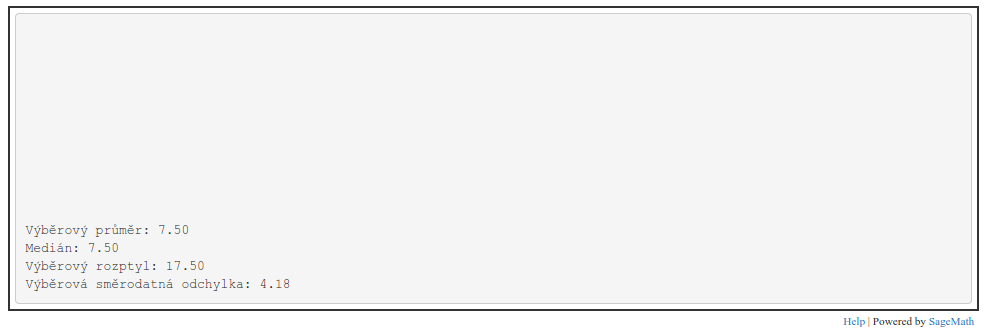
\includegraphics[scale=0.3]{grafics/sageRadky.png}
    \caption{Formátování výstupu kódu R v~buňce Sage Cell Server.}
\end{figure}

Použití jazyka Python také umožňuje využít příkaz \texttt{interact}, a tak usnadnit tvorbu interaktivních prvků aplikace. Ke statistickým výpočtům v~testovací aplikaci je vhodné použít knihovny Pythonu \textit{numpy}, \textit{scipy}, \textit{statsmodels} a \textit{matplotlib}. K~práci s~datovými soubory pak knihovnu \textit{urllib2}, která nám umožňuje jednoduše načítat data ze souborů. 


\subsection{Integrace}
Integrace modulů Sage do webové aplikace pomocí Sage Cell Server proběhla následovně:

\begin{enumerate}
\item Nejprve byly do HTML hlavičky stránky umístěny nutné tagy skript s~odkazem na~javascriptové knihovny jquery a Sage Cell Server. Do skriptu stránky pak byla umístěna funkce, která posléze mění objekty se zvolenou třídou (v našem případě objekty div se třidou compute) na~buňky Sage Cell Server. V~atributech této funkce bylo ponecháno výchozí nastavení pro~interpretaci kódu (jazyk Sage), ostaní nastavení bylo změněno tak, aby se kód automaticky vyhodnocoval při načtení stránky a aby bylo skryto vyhodnocovací tlačítko a zdrojový kód buněk.

\begin{verbatim}
sagecell.makeSagecell({inputLocation: 'div.compute',
                        template: sagecell.templates.minimal,
                        autoeval: true,
                        hide: ["evalButton",]});
    });
\end{verbatim}

\item Poté byly do těla dokumenty vloženy buňky (viz analýza) s~kódem Sage.
\end{enumerate}

\subsection{Implementace výpočtů}
%konkrétní funkce
\begin{sloppypar}

Načítání souborů v~Sage bylo provedeno pomocí knihovny \textit{urllib2} a její funkce \texttt{urlopen(url)}. 
Výpočty základních charakteristik veličin byly provedeny hlavně pomocí funkcí obsažených v~knihovně Pythonu \textit{numpy}, a to konkrétně \texttt{median(data)}, \texttt{mean(data)}, \texttt{cov(data1,data2)}, jenž funkcionalitou odpovídají stejnojmeným funkcím v~R. Dále byla použita funkce \texttt{var(data)} pro výpočet rozptylu, ta ovčem nepočítá bodový odhad výběrového rozptylu, a tak musel být výsledek upraven. Byla také použita funkce z~knihovny Pythonu \textit{scipy} \texttt{stats.pearsonr(data1, data2)} pro~výpočet korelačního koeficientu.   
Grafy byly vykresleny s~pomocí knihoven \textit{matplotlib}, \textit{numpy}, \textit{statsmodels} a \textit{scipy}, zároveň byl použit příkaz \texttt{interact}. 


\end{sloppypar}
\begin{enumerate}

\item \textbf{Histogram} \begin{sloppypar} Stejně jako v~R byly odhadnuty hodnoty pro~teoretická rozdělení metodou maximální věrohodnosti (viz analýza). Pro získání jeich hustoty pravděpodobnosti byly použity funkce \texttt{scipy.stats.norm.pdf}, \texttt{scipy.stats.expon.pdf}, \texttt{scipy.stats.uniform.pdf} s~příslušnými parametry. Samotný histogram pak byl vykreslen funkcí \texttt{matplotlib.pyplot.hist}.\end{sloppypar}

\item \textbf{Graf empirické distribuční funkce} \begin{sloppypar} Opět byly odhadnuty parametry teoretických rozdělení a jako parametry grafu poté použita funkce rozdělení získaná pomocí funkcí \texttt{scipy.stats.norm.cdf}, \texttt{scipy.stats.expon.cdf} a \texttt{scipy.stats.uniform.cdf}. Souhrnná empirická distribuční funkce byla spočítána pomocí funkce \texttt{statsmodels.api.distributions.ECDF(data)} a schodovitá křivka tohoto grafu vykreslena pomocí \texttt{matplotlib.pyplot.
step(data,ecdf(data)}. \end{sloppypar}

\item \textbf{Q-Q plot} \begin{sloppypar}V tomto případě byla pro~vykreslení grafu použita funkce \texttt{scipy.stats.problot}, jíž byly jako parametry předány odhadnuté parametry a název teoretického rozdělení, dále také zadaná data a objekt grafu, do něhož byla data vykreslena.\end{sloppypar}

\item \textbf{Scatter plot} \begin{sloppypar}Tento graf byl vykreslen pomocí funkce \texttt{matplotlib.pyplot.scatter(data1,data2)}.\end{sloppypar}

\end{enumerate}

\begin{sloppypar}
K testování hypotéz byly použity funkce z~knihovny \textit{scipy}. Konkrétně potom \texttt{stats.ttest\_1samp(data, null\_hypothesis)} pro~oboustranný jednovýběrový t-test o~střední hodnotě $\mu$, \texttt{stats.ttest\_rel(data1, data2)} pro~párový t-test o~rovnosti středních hodnot, pro~Kolmogorov-Smirnovův test dobré shody \texttt{stats.kstest(data, teorethical\_distribution)} pro~porovnání s~teoretickým rozdělením a \texttt{scipy.stats.ks\_2samp(data1,data2)} pro~porovnání dvou veličin. Použití těchto funkcí uživateli nedovoluje nastavit hladinu testu $\alpha$. Pro testování hypotéz bylo opět využito příkazu \texttt{interact}.  
\end{sloppypar}

\section{Srovnání systémů a vyhodnocení}
%rúzná rozhraní
Pro integraci prostředí R do webové stránky je možné využít mnoho nástrojů. Jedním z~nich je také API poskytované projektem OpenCPU. Od ostatních projektů se OpenCPU liší hlavně tím, že je kompatibilní s~jakýmkoliv jazykem či frameworkem, který umožňuje komunikaci pomocí protokolu HTTP. Další jeho přednost je, že vytváří pouze spojení mezi prostředím R a webovou aplikací a všechno ostatní je ponecháno na~uživateli. 

%a obtížnost/jednoduchost
Sage poskytuje k~integraci systému do webové stránky službu Sage Cell Server. Je to zatím jediné webové rozhraní pro~Sage, kromě přímé integrace Sage u~webových stránek postavených na~jazyce Python. Umožňuje nám jednoduchou možnost vložení buněk Sage do libovolné webové stránky a to pouze vložením několika skriptů v~jazyce javascript a tagů <div></div> se speciální třídou. Je tak umožněno, že kód může být vyhodnocen automaticky s~načtením stránky.

Použití systému OpenCPU je naproti tomu složitější. K~volání vlastních R funkcí je nutné vytvořit balíček R a umístit ho na~server poskytující tuto službu. Volání funkcí a manipulace s~jejich výstupy je pak prováděna pomocí HTTP požadavků GET a POST.

%open source, dokumentace
Oba systémy jsou Open Source a jsou tak uživatelům volně k~dispozici. Poskytují pro~použití veřejné servery nebo je uživateli umožněna instalace služby na~serveru vlastním, pro~což je u~obou k~dispozici podrobný návod a čas instalace je srovnatelný. Obě služby také uživatelům poskytují rozsáhlou dokumentaci včetně funkčních příkladů použití.

Služba Sage poskytuje pro~vyhodnocení buněk interprety různých jazyků, včetně pro~statistické výpočty vhodného jazyka R. Jejich použití však zdaleka nemusí být tak komfortní, jak jsou uživatelé u~těchto prostředí zvyklí. Veřejný server Sage Cell Server také zatím nepodporuje některé jejich funkcionality. 

%rúzné interprety /pouze R
OpenCPU je oproti tomu určeno pouze pro~jazyk R. Jeho použití však zachovává všechny funkcionality tohoto jazyka a kód R pro~použití API poskytované projektem OpenCPU není nutné nijak měnit.

%interact /statické R
Velkou výhodou Sage je příkaz \texttt{interact}. Ten uživateli umožňuje vkládat do svých modulů interaktivní prvky jako jsou posuvníky, zaškrtávací, textová a výběrová pole. To značně usnadňuje tvorbu modulů, kde je nutná interakce s~uživatelem.

Prostředí R je oproti tomu statické. OpenCPU API neposkytuje žádnou možnost vkládání interaktivních prvků. Ty lze ale ve stránce nahradit použitím jazyka PHP, nebo Javascriptu. Javascriptová knihovna opencpu poskytuje funkce usnadňující tvorbu interaktivních prvků ve webové stránce.

%nutnost mít výstup v~buňce, nemoci ho upravovat...javascript,php,... / volnost spravovat si vstupy i výstupy jak chce uživatel
Sage v~jistém smyslu omezuje svého uživatele nutností zobrazovat výstup ve výstupní buňce Sage. Veškeré jeho formátování je tedy nutné provádět v~jazyce, v~kterém je buňka interpretována. Výstupní buňky mají jednotný vzhled, jsou ohraničeny rámečkem s~odkazem na~domovskou stránku SageMath, který nelze skrýt.

OpenCPU naproti tomu nechává svému uživateli naprostou volnost ve zpracování výstupu. Id relace požadavku může být dokonce použito jako vstup dalšího volání funkce. Pro výstup lze zvolit velké množství formátů, mezi které patří také json, csv, png, svg a pdf, nebo lze použít výstup jako prostý text a jeho formátování provést v~jazyce webové aplikace. 

%komerční použití
Sage je šířen pod licencí GNU. Jednou z~podmínek této licence je, že případná díla odvozená musí být dále šířena také pod touto licencí. To sice úplně nevylučuje komerční šíření programu, je ale nutné v~tomto případě nechávat jeho kód opět volně k~dispozici. Pro cílového uživatele webové aplikace to také znamená nutnost potvrzovat souhlas s~licenčními podmínkami při vstupu na~stránku s~buňkami Sage.

OpenCPU je šířeno pod licencí Apache2, které narozdíl od licence GNU nepožaduje po uživateli copyleft. Uživatel tak nemusí modifikovaný program šířit opět pod stejnou licencí. Případná díla odvozená musí pouze zachovávat autorství nemodifikovaných částí, můžou však být použita buď jako open source nebo pro~komerční či akademické účely.

%statistické funkce
Jazyk a prostředí R jsou primárně určeny ke statistickým výpočtům a grafice. Poskytují tak k~tomuto účelu širokou škálu funkcí a rozšiřujících balíčků. K~základním statistickým výpočtům stačí využít standartní nabídku funkcí, není nutné instalovat žádné další balíčky.  

Jazyk Sage je určen obecně pro~matematické výpočty a geometrické experimentování. Některé knihovny jazyka Python poskytují základní statistické funkce. Jejich využití ale není tak konfortní, jako využití jazyka R a v~některých funkcích tak například nemáme tak široké možnosti nastavení jako v~prostředí R.

\begin{conclusion}
	%sem napište závěr Vaší práce
	%ÚVODNÍ VĚTA - NÁPLŇ (CÍL) PRÁCE; ZPŮSOB A MÍRA SPLNĚNÍ CÍLE(Ů); VÝHLED DO BUDOUCNA
Hlavním cílem práce bylo prozkoumat možnosti integrace volně dostupných matematických systémů R a Sage do~webových aplikací. Prvním cílem analytické části práce bylo analyzovat možností napojení statistického software R do webových aplikací, zvláště pak využitím API poskytovaného projektem OpenCPU a obdobně poté analyzovat možnosti napojení matematického software Sage, se zaměřením na~službu Sage Cell Server. Dalším cílem analytické části pak bylo prozkoumat závislost těchto řešení na~konkrétních webových technologiích. Cílem praktické části práce bylo navrhnout a vytvořit jednoduchou webovou aplikaci testující možnosti obou těchto systémů na~několika základních statistických úlohách. Na~závěr pak bylo cílem tato dvě řešení porovnat především z~hlediska praktické použitelnosti, efektivity a jednoduchosti integrace.

V první části práce byly nejprve analyzovány možnosti integrace R do webové aplikace také v~závislosti na~konkrétních webových technologiích. Poté byl rozebrán systém OpenCPU a popsány možnosti, které tento projekt nabízí. V~další části byl pak obdobně rozebrán projekt Sage a jeho služba pro~integraci do webové aplikace Sage Cell Server. Analytická část práce by se tak dala zhodnotit jako úspěšná. Bylo zjištěno, že systém OpenCPU není příliš závislý na~použitých webových technologiích, protože je kompatibilní s~jakýmkoliv frameworkem nebo jazykem, který umožňuje komunikaci pomocí protokolu HTTP. Také služba Sage Cell Server umožňuje vložení buněk Sage do libovolné webové stránky. 

K implementaci testovací aplikace byl zvolen jazyk PHP. Ve třetí části pak byla prozkoumána teorie k~výpočtům prováděným v~této aplikaci. Byla tak vytvořena jednoduchá interaktivní webová aplikace pro~základní statistické výpočty, která úspěšně integrovala systémy R i Sage. 

V závěrečné části práce byla porovnána řešení pomocí služby OpenCPU a Sage Cell Server. Bylo zjištěno, že velkou předností Sage je jednoduchost jeho integrace, dále pak možnost využítí různých interpretů pro~vyhodnocení kódu, ačkoliv ve webové aplikaci pouze s~omezenými možnostmi, a také příkaz \texttt{interact}. Přednostmi projektu OpenCPU jsou pak neomezené možnosti formátování výstupů, použitá licence, která umožňuje šířit modifikace bez nutnosti nechávat kód veřejně k~dispozici a pro~účely statistických výpočtů je to především možnost plnohodnotně použít jazyk R. Ukázalo se také, že integrace systému OpenCPU do webové aplikace je naproti Sage složitější a lze tak říci, že je z~hlediska praktické použitelnosti lepší systém Sage Cell Server. V~případě složitějších statistických výpočtů je pak ale vhodnější použít jazyk R a to se všemi možnostmi, které nabízí, a tak je vhodné použít systém OpenCPU. Ten byl také vyhodnocen jako efektivnější, díky způsobu, jakým spravuje relace. To funguje tak, že si server pamatuje id proběhlých relací a v~případě opětovného volání stejných požadavků nejsou funkce prováděny znovu, pouze je vráceno id relace, která již proběhla. Naproti tomu jsou buňky Sage opětovně vyhodnocovány po každém znovunačtení stránky. 

Hlavním přínosem práce je provedená analýza možností integrace systémů R a Sage do webové aplikace a porovnání obou provedených řešení, které pomohlo upozornit na~kladné i záporné vlastnosti obou systémů. Práce na~testovací aplikaci by mohla dále pokračovat implementací složitějších statistických úloh a mohla by se tak věnovat hlubší analýze možností použití obou systémů pro~statistické výpočty ve webových aplikacích. 
	
\end{conclusion}

\bibliographystyle{csn690}

\appendix

\begin{thebibliography}{Per00}

\bibitem[1]{statistika}
STIGLER, Stephen M.. \emph{The History of Statistics: The Measurement of Uncertainty before 1900.} Harvard : Belknap Press of Harvard University Press, 1990. ISBN 978-0674403413. 
 
\bibitem[2]{rproject.org-about}
\emph{R: What is R?} [online]. The R Foundation. [cit. 2015-04-26]. Dostupné z:  \url{http://www.r-project.org/} 

 \bibitem[3]{rproject.org} 
\emph{R-project} [online]. The R Foundation. [cit. 2015-04-26]. Dostupné z: \url{http://www.r-project.org/} 

 \bibitem[4]{rproject.org-webInterfaces}
\emph{R FAQ – R Web Interfaces} [online]. The R Foundation. [cit. 2015-04-26]. Dostupné z: \url{http://cran.r-project.org/doc/FAQ/R-FAQ.html\#R-Web-Interfaces}

 \bibitem[5]{Rweb}
\emph{Rweb} [online]. BANFIELD, Jeff. [cit. 2015-04-26]. Dostupné z: \url{http://www.math.montana.edu/Rweb/} 

 \bibitem[6]{RwebArticle}
BANFIELD, Jeff. Rweb: Web-based Statistical Analysis. \emph{Journal of Statistical Software} [online]. 1999, 1-15. ISSN 1548-7660. [cit. 2015-04-26]. Dostupné z: \url{http://www.jstatsoft.org/v04/i01/paper} 

 \bibitem[7]{RwebJean}
\emph{General Rweb interface} [online]. THIOULOUSE, Jean. (2008). [cit. 2015-04-26]. Dostupné z: \url{http://pbil.univ-lyon1.fr/Rweb/Rweb.general.html}

  \bibitem[8]{Ronline} 
\emph{Open Source Visions – R online} [online]. BARTEL, Ulf. (2002). [cit. 2015-04-26]. Dostupné z: \url{http://www.osvisions.com/r\_online/} 

 \bibitem[9]{WebDecomp}
\emph{Web Decomp} [online]. SATO, Seisho. [cit. 2015-04-26]. Dostupné z: \url{http://ssnt.ism.ac.jp/inets2/title.html}

 \bibitem[10]{Rserve} 
\emph{About Rserve} [online]. URBANEK, Simon. [cit. 2015-04-26]. Dostupné z: \url{http://rforge.net/Rserve/} 

 \bibitem[11]{FastRWeb} 
\emph{What is FastRWeb?} [online]. URBANEK, Simon. (2012). [cit. 2015-04-26]. Dostupné z: \url{http://rforge.net/FastRWeb/}

 \bibitem[12]{CGIwithRArticle}
FIRTH, David. CGIwithR: Facilities for processing web forms using R. \emph{Journal of Statistical Software} [online]. 2003, 1-8. ISSN 1548-7660. [cit. 2015-04-26]. Dostupné z: \url{http://www.jstatsoft.org/v08/i10/paper} 

 \bibitem[13]{CGIwithR}
\emph{CGIwithR package} [online]. FIRTH, David. (2014). [cit. 2015-04-26]. Dostupné z: \url{http://www.omegahat.org/CGIwithR/} 

 \bibitem[14]{slovnik}
KRAUS, Jiří et al. \emph{Nový akademický slovník cizích slov A-Ž.} Praha: ACADEMIA, 2007. ISBN 80-200-1415-2.

 \bibitem[15]{Rook}
\emph{Rook package} [online]. HORNER, Jeffrey. (2014). [cit. 2015-04-27]. Dostupné z: \url{http://cran.r-project.org/web/packages/Rook/Rook.pdf} 

\bibitem[16]{RApache}
\emph{Web Application Development with R and Apache} [online]. Vanderbilt University. (2013). [cit. 2015-04-27]. 
Dostupné z: \url{http://rapache.net/index.html}

\bibitem[17]{brew}
\emph{Package brew} [online]. HORNER, Jeffrey. (2010). [cit. 2015-04-27]. Dostupné z: \url{http://cran.r-project.org/web/packages/brew/brew.pdf} 

 \bibitem[18]{Rwui}
\emph{Rwui: A web application to create user 
friendly web interfaces for R scripts} [online]. NEWTON, R., WERNISCH, L.. [cit. 2015-04-27]. Dostupné z: \url{http://sysbio.mrc-bsu.cam.ac.uk/Rwui/tutorial/Rwui\_Rnews\_final.pdf}

 \bibitem[19]{R-php}
\emph{R-php} [online]. PONTILLO, Alfredo, MINEO, Angelo. (2005). [cit. 2015-04-27]. Dostupné z: \url{http://dssm.unipa.it/R-php/?cmd=home}

 \bibitem[20]{R_PHP_ONLINE}
\emph{R\_PHP\_ONLINE} [online]. Steve Chen. (2003). [cit. 2015-04-27]. Dostupné z: \url{http://steve-chen.net/document/r/r\_php}

\bibitem[21]{Shiny}
\emph{Shiny} [online]. RStudio. (2014). [cit. 2015-04-27]. Dostupné z: \url{http://shiny.rstudio.com/}

\bibitem[22]{OpenCPU-Papers}
\emph{OpenCPU – Papers} [online]. OpenCPU. (2013). [cit. 2015-04-27]. Dostupné z: \url{https://www.opencpu.org/papers.html}

\bibitem[23]{OpenCPUreaease146}
OOMS, Jeroen. OpenCPU release 1.4.6: gzip and systemd. \emph{OpenCPU} [online]. OpenCPU, 2014. [cit. 2015-04-27]. 
Dostupné z: \url{https://www.opencpu.org/posts/opencpu-release-1-4-6/}

\bibitem[24]{OpenCPUjsLibrary}
\emph{OpenCPU – JavaScript Client} [online]. OpenCPU. (2014). [cit. 2015-04-27]. Dostupné z: \url{https://www.opencpu.org/jslib.html}

\bibitem[25]{info}
\emph{Information on package ’A3’} [online]. OOMS, Jeroen. (2013). [cit. 2015-04-27]. Dostupné z: \url{https://demo.ocpu.io/A3/info}

\bibitem[26]{RPackageWriting}
\emph{Writing R Extensions} [online]. The R Foundation. [cit. 2015-04-27]. Dostupné z: \url{http://cran.r-project.org/doc/manuals/r-release/R-exts.html\#Creating-R-packages}

\bibitem[27]{OpenCPUwebhook}
\emph{OpenCPU – API Docs} [online]. OpenCPU. [cit. 2015-04-27]. Dostupné z: \url{https://www.opencpu.org/api.html\#api-ci}

\bibitem[28]{SageIntro}
\emph{SageMath} [online]. SageMath Mathematical Software. [cit. 2015-04-27]. 
Dostupné z: \url{http://www.sagemath.org/}

\bibitem[29]{FoCM2011}
STEIN, William. Sage - Creating a viable free open source alternative to Magma,
Maple, Mathematica and Matlab. In: \emph{Foundations of Computational Mathematics, 
Budapest 2011.}
Cambridge, England: Cambridge University Press, 2012. ISBN 9781107604070.

\bibitem[30]{tracSage}
\emph{Sage Developer Trac} [online]. SageMath Mathematical Software. (2015). [cit. 2015-04-26]. Dostupné z: \url{http://trac.sagemath.org/}

\bibitem[31]{Cython}
\emph{About Cython} [online]. [cit. 2015-05-01]. Dostupné z: \url{http://cython.org/\#about}

\bibitem[32]{SageCloud}
\emph{SageMathCloud} [online]. SageMathCloud. [cit. 2015-04-26]. Dostupné z: \url{https://cloud.sagemath.com/}

\bibitem[33]{SageInterfaces}
\emph{Interpreter Interfaces} [online]. The Sage Development Team. (2005 – 2015). [cit. 2015-04-26]. Dostupné z: \url{http://www.sagemath.org/doc/reference/interfaces/}

\bibitem[34]{SageInteract}
\emph{Interact – Sage Wiki} [online]. [cit. 2015-05-01]. Dostupné z: \url{http://wiki.sagemath.org/interact/}

\bibitem[35]{SageCellServer}
\emph{About the Sage Cell Server} [online]. (2011). [cit. 2015-05-01]. Dostupné z: \url{http://sagecell.sagemath.org/static/
about.html?v=15adefe8b7e89fcf49eda7af5303abd4}

\bibitem[36]{CodingCython}
\emph{Coding in Cython – Sage Developer’s Guide v6.6.beta0} [online]. The Sage Development Team. (2005 – 2015). [cit. 2015-05-01]. Dostupné z: \url{http://www.sagemath.org/doc/developer/coding\_in\_cython.html}

\bibitem[37]{random}
\emph{Generate pseudo-random numbers} [online]. Python Software Foundation. (1990-2015). [cit. 2015-04-26]. Dostupné z: \url{https://docs.python.org/3.4/library/random.html}

\bibitem[38]{statistics}
\emph{Mathematical statistics functions} [online]. Python Software Foundation. (1990-2015). [cit. 2015-04-26]. Dostupné z: \url{https://docs.python.org/3/library/statistics.html}

\bibitem[39]{SciPy}
\emph{Scientific Computing Tools for Python – SciPy.org} [online]. SciPy developers. (2015). [cit. 2015-04-26]. Dostupné z: \url{http://www.scipy.org/about.html}

\bibitem[40]{NumPy}
\emph{NumPy} [online]. Numpy developers. (2013). [cit. 2015-04-26]. Dostupné z: \url{http://www.numpy.org/}

\bibitem[41]{matplotlib}
\emph{matplotlib: python plotting} [online]. HUNTER, John et al.. (2002-2012). [cit. 2015-04-26]. Dostupné z: \url{http://matplotlib.org/}

\bibitem[42]{IPython}
\emph{Jupyter and the future of IPython} [online]. IPython development team. (2015). [cit. 2015-04-26]. Dostupné z: \url{http://ipython.org/}

\bibitem[43]{pandas}
\emph{pandas: Python Data Analysis Library} [online]. Python Data Analysis Library. (2015). [cit. 2015-04-26]. Dostupné z: \url{http://pandas.pydata.org/}

\bibitem[44]{rpy2}
\emph{rpy2.} [online]. GAUTIER, L.. (2014). [cit. 2015-04-26]. Dostupné z: \url{http://rpy.sourceforge.net/}

\bibitem[45]{statlib}
\emph{python-statlib – descriptive statistics for the python programming language} [online]. Google Project Hosting. (2007). [cit. 2015-04-26]. Dostupné z: \url{https://code.google.com/p/python-statlib/}

\bibitem[46]{StatsDoc}
\emph{StatsDoc – python-statlib – documentation for the stats module.} [online]. Google Project Hosting. [cit. 2015-04-26]. Dostupné z: \url{https://code.google.com/p/python-statlib/wiki/StatsDoc}

\bibitem[47]{PstatDoc}
\emph{PstatDoc – python-statlib – documentation for the pstat module.} [online]. Google Project Hosting. [cit. 2015-04-26]. Dostupné z: \url{https://code.google.com/p/python-statlib/wiki/PstatDoc}

\bibitem[48]{Matfunc}
\emph{Documentation for MATFUNC.} [online]. HETTINGER, Raymond. (2001). [cit. 2015-04-26]. Dostupné z: \url{http://users.rcn.com/python/download/matfunc.htm}

\bibitem[49]{statsmodels}
\emph{StatsModels: Statistics in Python} [online]. The Statsmodels Development Team. (2012). [cit. 2015-04-26]. Dostupné z: \url{http://statsmodels.sourceforge.net/}

\bibitem[50]{PyMC}
\emph{Introduction} [online]. FONNESBECK, Christopher J.. (2014). [cit. 2015-04-26]. Dostupné z: \url{https://pymc-devs.github.io/pymc/README.html}

\bibitem[51]{PyMix}
\emph{PyMix/home} [online]. [cit. 2015-04-26]. Dostupné z: \url{http://www.pymix.org/pymix/}

\bibitem[52]{sagemathGithub}
\emph{sagemath/sagecell} [online]. [cit. 2015-04-26]. Dostupné z: \url{https://github.com/sagemath/sagecell}

\bibitem[53]{Anděl}
ANDĚL, Jiří. \emph{Základy matematické statistiky.} Druhé upravené vydání. Praha: MATFYZPRESS, 2007. ISBN 80-7378-001-1.

\bibitem[54]{VŠCHT}
PAVLÍK, Jiří et al. \emph{Aplikovaná statistika.} Praha: VŠCHT Praha, 2005. ISBN 80-7080-569-2.

\bibitem[55]{GraphMethods}
CHAMBERS, John M. et al. \emph{Graphical methods for data analysis.} New Jersey: Wadsworth \& Brooks, 1983. ISBN 0-534-98052.

\bibitem[56]{PHP}
\emph{Usage Statistics and Market Share of Server-side Programming Languages for Websites.} [online]. W3Techs. (2015). [cit. 2015-05-10]. Dostupné z: \url{http://w3techs.com/technologies/overview/programming\_language/all}

\end{thebibliography}

\chapter{Seznam použitých zkratek}
%\printglossaries
\begin{description}
    \item[AJAX] Asynchronous JavaScript and XML
    \item[API] Application Programming Interface
	\item[CAS] Computer Algebra System
	\item[CDF] Cumulative Distribution Function
    \item[CGI] Common Gateway Interface
    \item[CORS] Cross Domain OpenCPU Request
    \item[CRAN] Comprehensive R Archive Network
    \item[CSS] Cascading Style Sheets
    \item[CSV] Comma-Separated Values
    \item[cURL] client URL Library
    \item[FAQ] Frequently Asked Questions
    \item[GNU] General Public License
    \item[GPL] General Public License
    \item[HTML] Hypertext Markup Language
    \item[HTTP] Hypertext Transfer Protocol
    \item[HTTPS] Hypertext Transfer Protocol Secure
    \item[IRT] Item Response Theory
    \item[JSON] JavaScript Object Notation
    \item[MLE] Maximum Likelihood Estimation
    \item[PHP] Hypertext Preprocessor
    \item[Q-Q plot] Quantile-Quantile plot
    \item[RPC] Remote Procedure Call
    \item[SSL] Secure Sockets Layer
\end{description}

\chapter{Obsah přiloženého CD}

%upravte podle skutecnosti

\begin{figure}
	\dirtree{%
		.1 readme.txt\DTcomment{stručný popis obsahu CD}.
		.1 www\DTcomment{adresář se zdrojovými kódy webové aplikace}.
		.2 img\DTcomment{obrázky do webových stránek}.
		.2 css\DTcomment{kaskádové styly aplikace}.
		.2 *\DTcomment{PHP stránky a potřebné javascriptové knihovny}.
		.1 src.
		.2 newPackage\DTcomment{balíček R funkcí}.
		.2 data\DTcomment{data ve formátu CSV pro testování aplikace}.
		.2 text\DTcomment{soubory k vygenerování textu práce}.
		.3 BP\_Ernekerová\_Jana\_2015.tex\DTcomment{zdrojová forma práce ve formátu \LaTeX{}}.
		.3 *\DTcomment{ostatní soubory šablony potřebné k vygenerování práce}.
		.1 text\DTcomment{text práce}.
		.2 BP\_Ernekerová\_Jana\_2015.pdf\DTcomment{text práce ve formátu PDF}.
	}
\end{figure}

\end{document}
